%%% Additions / Corrections
%%%  Add a problem that relates geometry to complex numbers -- perhaps the median concurrency
%%% Use complex numbers to get the double angle formulas
%%% In problem 84, use the half-angle formula to figure out what the number is.

%%% Or, the perpendicular bisector
%%% Phasors still need some clarification %%%
%%% Make complex diagram %%%

%%%%(c)
%%%%(c)  This file is a portion of the source for the textbook
%%%%(c)
%%%%(c)    Abstract Algebra: Theory and Applications
%%%%(c)    Copyright 1997 by Thomas W. Judson
%%%%(c)
%%%%(c)  See the file COPYING.txt for copying conditions
%%%%(c)
%%%%(c)
\chap{Complex Numbers}{complex}

\begin{dialogue}
\speak{Horatio} O day and night, but this is wondrous strange!
\speak{Hamlet} And therefore as a stranger give it welcome.
There are more things in heaven and earth, Horatio,
Than are dreamt of in your philosophy.
\noindent
\end{dialogue}
(Source: Shakespeare, \emph{Hamlet}, Act 1 Scene 5.)
\bigskip

\bigskip

Although complex numbers are defined to include ``imaginary'' numbers, the practical applications of complex numbers are far from ``imaginary''.  We shall touch on some of the applications in this chapter: but there are many many more in engineering, in physics, and in other sciences as well.
\medskip

Thanks to Tom Judson for material used in this chapter.

\section{The origin of complex numbers\quad\sectionvideohref{yhSLFJJZ9us&index=3&list=PL2uooHqQ6T7PW5na4EX8rQX2WvBBdM8Qo}}
\label{sec:origin_complex}

\subsection{A number that can't be real (and we can prove it!)}

Way back in your first algebra class, you saw equations like:
\begin{itemize}
\item $x^2 = 4$
\item $x^2 = 36$
\item $x^2 = 7$

\end{itemize}
You also learned how to solve them either by hand, or using the \texttt{SQRT} button on a simple calculator. The solutions to these equations are
\begin{itemize}
\item $x = \pm 2$
\item $x = \pm 6$
\item $x = \pm 2.64575131106459\ldots$
\end{itemize}
 But what about equations like:
\[x^2 = -1 \]
Your simple calculator can't help you with that one!\footnote{It's true that the fancier graphing calculators can handle it, but that's beside the point.}  If you try to take the square root of -1, the calculator will choke out \texttt{ERR OR} or some similar message of distress.  But why does it do this? Doesn't $-1$ have a square root? 

In fact, we can prove mathematically that $-1$ does not have a \emph{real} square root. As proofs will play a very important part in this course, we'll spend some extra time and care explaining this first proof.

\begin{prop}{no_sqrt} $-1$ has no real square root.
\end{prop}
\begin{proof}
We give two proofs of this proposition. The first one explains all
the details, while the second proof is more streamlined. It is the streamlined
proof that you should try to imitate when you write up proofs for
homework exercises.
\medskip{}
\newline
\noindent \textbf{Long drawn-out proof of Proposition~\ref{proposition:complex:no_sqrt} with all the gory details:} 

We will use a common proof technique called {\bf \emph{ proof by contradiction}}\index{Proof by contradiction}. 
Here's how it goes:

First we \emph{suppose} that there exists a real number \emph{a} such that
$a^{2}=-1$. Now we know that any real number is either positive, or zero, or negative$-$there are no other possibilities. So we consider each of these three cases: $a>0,$ or $a=0,$ or $a<0$.

\begin{itemize}
\item
In the case that $a>0$ then $a^{2}= a\cdot a =$ (\emph{positive})$\cdot$(\emph{positive})
= a positive number (that is, $a^{2}>0$). But this couldn't possibly
be true, because we have already supposed that $a^{2}=-1$: there's
no way that $a^{2}>0$ and $a^{2}=-1$ can both be true at the same
time!

\item
In the case that $a=0$, then $a^{2}=a\cdot a = (0)\cdot(0)
= 0$. But $a^{2}=0$ also contradicts our \emph{supposition} that $a^{2}=-1$.
\item
In the case that $a<0$, then $a^{2}$= $a\cdot a$ = (\emph{negative})$\cdot$(\emph{negative})
= a positive number, so $a^{2}>0$. As in the first case, this contradicts
our \emph{supposition} that $a^{2}=-1$.
\end{itemize}

So no matter which of the three possible cases is true, we're still
screwed: in every case, we always have a contradiction. We seem to have reached a dead end -- a logically impossible conclusion. So what's wrong?

What's wrong is the \emph{supposition}. It \underbar{must} be the case that the supposition is not
true. Consequently, the statement ``there exists a real number
\emph{a} such that $a^{2}=-1$'' must be \underbar{false}. In other
words, $-1$ has no real square root. This completes the proof. $\square$
\footnote{The '$\square$' symbol will be used to indicate the end of a proof. In other words: Ta-da!}
\medskip{}
\newline
The above proof is pretty wordy. Often the first draft of a proof can be pretty messy. So it's usually good to go back and rewrite the proof in such a  way as to bring out the essential details. Here's our second crack at the above proof:
\medskip{}
\newline
\noindent \textbf{Streamlined proof of Proposition~\ref{proposition:complex:no_sqrt} (suitable for writing up homework exercises)}

The proof is by contradiction. Suppose $\exists \emph{a} \in \mathbb{R}$
such that $a^{2}=-1$ (note the symbol ``$\exists$" means ``there exists,'' the symbol $\mathbb{R}$ denotes the real numbers, and the expression ``$\emph{a} \in \mathbb{R}$'' means that $a$ is contained in $\mathbb{R}$, that is, $a$ is a real number).

There are two cases: either (i) $a\geq0$ or (ii) $a<0$.

In Case (i), then $a^{2}$= \emph{$a\cdot a$ =} (\emph{nonnegative})$\cdot$(\emph{nonnegative})
$\geqq0$, which contradicts the supposition.

In Case (ii), then $a^{2}$= \emph{$a\cdot a$ =} (\emph{negative})$\cdot$(\emph{negative})
$>0$, which contradicts the supposition.

By contradiction, it follows that $-1$ has no real square root.
\end{proof}
You may note that in the streamlined case, we reduced the number of cases from three to two.  That's because we noticed that we really could combine the ``positive'' and the ``zero'' case into a single case.

So far we've only considered square roots, but naturally we may ask the same questions about cube roots, fourth roots, and so on: 

\begin{exercise}{root1}
 Imitate the proof of Proposition~\ref{proposition:complex:no_sqrt} to prove that $-2$ has no real fourth root.
\end{exercise}

\begin{exercise}{root2}
Try to use the method of Proposition~\ref{proposition:complex:no_sqrt} to prove that -4 has no real cube root. At what step does the method fail?
\end{exercise}

Notice that the $n$th root of $a$ is a solution of the equation $x^n - a=0$ (and conversely--any solution of $x^n- a=0$ is an $n$th root of $a$). 
Based on this observation, we may generalize the notion of ``root'':

\begin{defn} Given a function $f(x)$ which is defined on the real numbers and takes real values, then a \term*{root}\index{Root! of a real function} of $f(x)$ is any solution of the equation $f(x)=0$.  
\end{defn}

\begin{exercise}{graph}
\begin{enumerate}[(a)]
\item
Sketch the function  $f(x) = x^2 + 9$. Does the function have any real roots? Explain how you can use the graph to answer this question.
\item 
Prove that the function $f(x) = x^2 + 9$ has no real roots.  (You may prove by contradiction, as before). 
\item
Graph the function $f(x) = x^6 + 7x^2 + 5$ (you may use a graphing calculator). Determine whether $f(x)$ has any real roots. \emph{Prove} your answer (note: a picture is not a proof!).
\end{enumerate}
\end{exercise}
\noindent
Exercise~\ref{exercise:complex:graph} underscores an important point. A graph can be a good visual aid, but it's not a mathematical proof.  We will often use pictures and graphs to clarify things, but in the end we're only certain of what we can prove. After all, pictures can be misleading.

\begin{exercise}{more}
*\footnote{Asterisks (*) indicate problems that are more difficult. Take the challenge!}~~Suppose that $a \cdot x^{2n} + b \cdot x^{2m} +a = 0$ has a real root, where $a,b,m,n$ are nonzero integers. What can you conclude about the signs of $a$ and $b$? \emph{Prove} your answer.
\end{exercise}

\subsection{Unreal, but unavoidable}

Mathematicians have known Proposition~\ref{proposition:complex:no_sqrt} for thousands of years, and
for a long time that settled the question. Unfortunately, that nasty
$\sqrt{-1}$ kept popping up in all sorts of inconvenient places.
For example, about 400 years ago, it was very fashionable to study
the roots of cubic polynomials such as $x^{3}-15x-4=0$. A mathematician
named Bombelli came up with a formula for a solution that eventually
simplified to: $x = (2 + \sqrt{-1}) + (2 - \sqrt{-1})$. By canceling
out the $\sqrt{-1}$ terms, he got the correct solution $x=4$.
But how can you cancel something that doesn't exist?

Since mathematicians couldn't completely avoid those embarrassing 
$\sqrt{-1}$'s, they decided to put up with them as best they could. They
called $\sqrt{-1}$ an \emph{imaginary} number\index{Imaginary number}, just to emphasize
that it wasn't up to par with the \emph{real} numbers. They also used the symbol $i$ to represent $\sqrt{-1}$, to make it less
conspicuous (and easier to write). Finally, they created a larger
set of numbers that included both real and imaginary numbers, called
the \emph{complex numbers.}\index{Complex numbers!definition of}
\footnote{The web site http://math.fullerton.edu/mathews/n2003/ComplexNumberOrigin.html
gives more information about the origin of complex numbers.}

\begin{defn}
The \term{complex numbers}\index{Complex numbers!definition} are defined
as 
\[
{\mathbb{C}}=\{a+bi:a,b\in{\mathbb{R}}\},\]
 where $i^{2}=-1$. If $z=a+bi$, then $a$ is the \term{real
part}\index{Complex numbers!real part} of $z$ and $b$ is the \term{imaginary part}\index{Complex numbers!imaginary part}\index{Imaginary part} of $z$. (Note that the imaginary part of a complex number is a \emph{real number}. It is the coefficient of $i$ in the expression $z = a + bi$.)
\end{defn}

\bigskip

 Examples of complex numbers include 
\begin{itemize}
\item 1 + $i$ 
\item $5.387-6.432i$ 
\item $\frac{1}{2}-\frac{\sqrt{3}}{2}i$ 
\item $3i$ (equal to $0+3i$) 
\item 7.42 (equal to $7.42+0i$).
\item 0 (equal to $0+0i$).
\end{itemize}
\begin{exercise}{1}
\begin{enumerate}[(a)]
\item
Write down the complex number with real part 0 and imaginary part 7.
\item
Write down a complex number whose real part is the negative of its imaginary part.
\item
Write down a complex number that is also a real number.
\end{enumerate}
\end{exercise}

\subsection{A mathematical revolution}

The creation of complex numbers was a revolutionary event in
the history of mathematics. Mathematicians were forced to recognize
that their beloved ``real'' numbers just weren't good enough to
deal with the mathematical problems they were encountering. So they
had to create a \emph{new} \emph{number system} (the complex numbers)
with\emph{ new}  symbols ($i$) and \emph{new} arithmetic rules
(like $i\cdot i=-1$).

In fact, this was not the first time that a controversial new number
system was founded. The ancient Greeks thought that all numbers could
be expressed as a ratio of integers $\frac{m}{n}$ --- in other words, the Greeks thought all numbers were rational.  It came as a huge
shock when someone proved that some real numbers are \emph{not} rational. We will presently give the original proof, but first we will need some properties of odd and even integers:

\begin{exercise}{m2even}
\begin{enumerate}[(a)]
\item
Fill in the blanks:  The product of two odd integers is $\underline{~<1>~}$ , and the product of two even integers is $\underline{~<2>~}$ .
\item
Use proof by contradiction to prove the following statement: If $m$ is an integer and $m^2$ is even, then $m$ is also even.
%(\emph{Hint}: see \ref{sec:complex:hints})
\hyperref[sec:complex:hints]{(*Hint*)}\footnote{All *Hints* can be found at the end of the book (or by clicking on the *Hints* link.)}
\item 
It is possible to make a more general statement than part (b).Use proof by contradiction to prove the following statement: If $m$ is an integer $d$ is a positive integer, and $m^d$ is even, then $m$ is also even. 
\hyperref[sec:complex:hints]{(*Hint*)}
\end{enumerate}
\end{exercise}

\begin{prop}{irrational}
Given a right isosceles triangle where both legs have length 1 (see Figure~\ref{fig:complex:isosceles_right}) .  Let $x$ be the length of the hypotenuse.  Then $x$ is irrational--that is, it cannot be expressed as a ratio of integers.\index{Irrational number!definition of} 
\end{prop}
\begin{figure}[htb]
	   \center{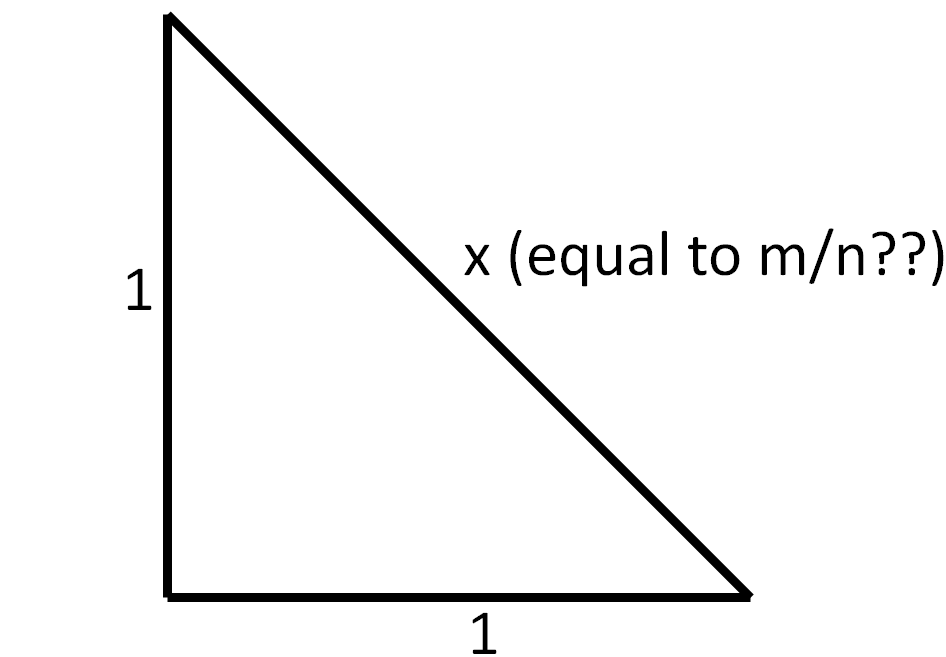
\includegraphics[width=2in]
	         {images/isosceles_right.png}}
	  \caption{\label{fig:complex:isosceles_right} Isosceles right triangle }
\end{figure}

\begin{proof}
The proof is by contradiction.\index{Irrational number!existence proof}   \emph{Suppose} that $x$ is rational: that is, $x = \frac{m}{n}$ for some integers $m$ and $n$.We can always reduce a fraction to lowest terms ( as noted in Section~\ref{subsec:eqsAndIneqs}), so we can assume $m$ and $n$ have no common factors. 

Since $x$ is the hypotenuse of a right triangle, the Pythagorean Theorem gives us $x^2 = 1^2 + 1^2 = 2$.
We can plug $x=\frac{m}{n}$ into $x^2 = 2$ to get $\left(\frac{m}{n}\right) ^2 = 2$, which can be rearranged to give 
\[ m^2 = 2n^2.\]
From this we see that $m^2$  is divisible by 2, which means that $m^2$ is even. Exercise~\ref{exercise:complex:m2even} part (b) then tells us that $m$ is even, so there must be an integer $j$ such that  $m = 2j$.  Plugging $m=2j$ into $m^2=2n^2$  gives $4j^2 = 2n^2$, which simplifies to $2j^2 = n^2$.  Hence $ n^2$ is even, and as before we conclude that $n$ is even.  So $n = 2k$ for some integer $k$.

At this point, we have $m = 2j$ and $n = 2k$, which means that $m$ and $n$ have a common factor of 2.  But at the beginning of the proof, we said that  $m$ and $n$ were reduced to lowest terms, so they  have no common factor.  This is a contradiction.  Therefore our \emph{supposition} must be false, so $x$ cannot be rational.
\end{proof}

We have seen in our proofs that whenever we make a statement, we also need to give a reason that justifies the statement. In many cases, it's possible to state a proof very succinctly in  ``statement$-$reason'' format.\index{Proofs!``statement$-$reason'' format} For instance, here is a ``statement$-$reason'' proof of Proposition~\ref{proposition:complex:irrational}:

\begin{tabular}{l| l}
Statement& Reason\\
\hline
$x$ is the hypotenuse of the right & Given\\
~~ triangle in Figure~\ref{fig:complex:isosceles_right} & ~\\
$x$ is rational & \emph{supposition} (will be contradicted)\\
$x^2 = 2$ & Pythagorean Theorem\\
$x = m/n$ where $m,n$ are integers& Definition of rational\\
$m, n$ have no common factors & Fraction can always be reduced\\
$(m/n)^2 = 2$ & Substitution\\
$m^2 = 2n^2$ & Rearrangement\\
$m = 2k$ where $k$ is an integer & Exercise~\ref{exercise:complex:m2even} part (b)\\
$(2k/n)^2 = 2$ & Substitution\\
$n^2 = 2k^2$& Rearrangement\\
$n = 2j$ where  $j$ is an integer&Exercise~\ref{exercise:complex:m2even} part (b)\\
$m$ and $n$ have a common factor& 2 is a factor of both\\
\emph{supposition} is false & Contradictory statements\\
$x$ cannot be rational &  Negation of supposition
\end{tabular}

Note that the preceding proof amounts to a proof that $\sqrt{2}$ is irrational, since we know that $\sqrt{2}$ is the length of the hypothesis in question. Given the results of Exercise~\ref{exercise:complex:m2even}, we can use a similar proof to find more irrational numbers.

\begin{exercise}{6}
\begin{enumerate}[(a)]
\item
Prove that the cube root of 2 is irrational.
\hyperref[sec:complex:hints]{(*Hint*)} 
\item
Prove that the $n$th root of 2 is irrational, if $n$ is a positive integer greater than 1.
\item
Prove that $2^{1/n}$ is irrational, if $n$ is a negative integer less than -1.
\end{enumerate}
\end{exercise}

In the proof of Proposition~\ref{proposition:complex:irrational},  we ``plugged in'' or substituted one expression for another.   For example, when we discovered that $m$ was divisible by 2 we substituted $2j$ for $m$, which was useful for the algebra that followed.
\emph{Substitution}\index{Substitution!as proof technique} is a key technique used throughout all of abstract algebra.

\begin{exercise}{2}
Use substitution to prove the following statement:  if $3 | n$ and $4 | m$, then $12 | mn$ (the notation ``$3 | n$'' means that 3 divides $n$). 
\hyperref[sec:complex:hints]{(*Hint*)}
\end{exercise}

\begin{exercise}{3}
Use substitution to prove the following statement:  if $12 | n$ and $n | 4m$, where $n$ and $m$ are integers, then $3 | m$.
\hyperref[sec:complex:hints]{(*Hint*)}
\end{exercise}

We should also come clean and admit that our proof of Proposition~\ref{proposition:complex:irrational} falls short of true mathematical rigor. The reason is that we made use of Exercise~\ref{exercise:complex:m2even}, and we never actually proved part (a) of the exercise. Even though it's something that ``everybody knows", mathematicians still want a proof! Now, part (a) is a consequence of a more general proposition known as \term{Euclid's Lemma}:\index{Euclid's lemma}. Before giving this lemma, let's be precise about what we mean by ``prime number'':

\begin{defn}\label{defPrime} A \term*{prime number}\index{Prime!definition} is a natural number (i.e. positive integer) bigger than 1 that only has one factor bigger than 1, namely itself.
\end{defn}

Now we are ready to state Euclid's lemma: 

\begin{prop}{EuclidLemma}
Let $a$ and $b$ be integers, and let $p$ be a prime number. If $p$ divides $ab$, then either $p$ divides $a$, or $p$ divides $b$.

\begin{rem}
In mathematics, when we say ``either X is true or Y is true'', we also include the possibility that both X and Y are true. So in this case, when we say ``$p$ divides $a$, or $p$ divides $b$'', it's possible that $p$ divides both $a$ and $b$.
\end{rem}

\end{prop}
\begin{proof}
We're not ready to give a proof yet, but we'll give one later (see Exercise~\ref{exercise:modular:EuclidLemmaProof}  in Section~\ref{sec:diophantine}).
\end{proof}


\begin{exercise}{4}
Modify the proof of Proposition~\ref{proposition:complex:irrational} to prove that $\sqrt{3}$ is irrational. (You will find Proposition~\ref{proposition:complex:EuclidLemma} to be useful in the proof.)
\end{exercise}

\begin{exercise}{5}
Prove that $\sqrt{6}$ is irrational.
\end{exercise}

\begin{exercise}{6a}
Prove that $p^{1/n}$ is irrational, if $p$ is a prime and $n$ is any integer with $|n|>1$.
\end{exercise}

\begin{exercise}{6aa}
\begin{enumerate}[(a)]
\item
Suppose that $a,b,c$ are integers and  $(a/b)^2 = c$.  Suppose further that $a$ and $b$ have no common factors except $1$: that is, any integer $x > 1$ which divides $b$ doesn't divide $a$.  Prove by contradiction that $b=1$.
\item
Generalize part (a): Suppose that $a,b,c$ are integers and  $(a/b)^n = c$, where $n$ is a positive integer. If $a$ and $b$ have no common factors, prove by contradiction that $b=1$.
\item
Use part (b) to prove the following: Let $a$ and $n$ be integers, both greater than 1. Let $x$ be a real $n$th root of $a$.  If $x$ is not an integer, then $x$ is irrational.
\end{enumerate}
\end{exercise}


The inconvenient truth expressed in Proposition~\ref{proposition:complex:irrational} forced mathematicians to extend
the 'real' numbers to include \emph{irrational} as well as \emph{rational}
numbers. But complex numbers opened the floodgates by setting a precedent. New generations of mathematicians 
became so used to working with ``unreal'' numbers that they became accustomed to making up other number systems whenever it suited their purpose.
Within a few centuries after the complex numbers, several new
number systems were created. This eventually prompted  mathematicians to study the properties of general numbers
systems. The outcome of this is what is known today as  abstract
algebra!

To close this section, here's another exercise to practice using substitution:

\begin{exercise}{root3}
\begin{enumerate}[(a)]
\item
Suppose that:
\begin{itemize}
\item
$a$ is a negative number;
\item
$n$ is a positive integer;
\item
the equation $x^n = a$ has a real solution for the unknown $x$.
\end{itemize}
What can you conclude about $n$? Make a clear statement and \emph{prove} your statement.
\hyperref[sec:complex:hints]{(*Hint*)}

\item
Replace the condition ``$n$ is a positive integer'' in part (a) with ``$n$ is a negative integer.'' Now what can you conclude about $n$? Make a clear statement and \emph{prove} your statement.
\end{enumerate}
\end{exercise}


\begin{exercise}{7} Do imaginary numbers ``really'' exist? Write
two or three sentences to express your opinion.\footnote{There is no ``right'' answer to this question.}
\end{exercise}


\section{Arithmetic with complex numbers\quad 
\sectionvideohref{xok7xHQuTzU&list=PL2uooHqQ6T7PW5na4EX8rQX2WvBBdM8Qo&index=4}}
\label{sec:complex_arith}

\subsection{Complex arithmetic}

To add \index{Complex numbers!addition}two complex numbers $z=a+bi$ and $w=c+di$, we just add the
corresponding real and imaginary parts: 
\[(a+bi)+(c+di)=(a+c)+(b+d)i.\]
Using this definition, we may prove directly that complex addition (like regular addition) is commutative:\footnote{It is important to realize that this \emph{must} be proved and \emph{can't} just be assumed.  Later on we will define operations that are \emph{not} commutative.}

\begin{prop}{complex_comm}
Addition on complex numbers is commutative.
\end{prop}
\begin{proof}
We just need to show that for any two complex numbers $z$ and $w$, it's always true that $z + w = w + z$.  Writing $z = a + bi$ and $w = c + di$ as above, the proof using statement-reason format runs as follows:

\begin{tabular}{l| l}
Statement& Reason\\
\hline
$z + w = (a + bi) + (c + di)$ &substitution\\
~~~~~~ $= (a + c) + (b + d)i$ & definition of complex addition\\
~~~~~~ $= (c + a) + (d + b)i$ & real addition is commutative\\
~~~~~~ $= (c + di) + (a + bi)$ & def. of complex addition\\
~~~~~~ $= w + z$. & substitution\\
\end{tabular}

\end{proof}

Notice how we started in this proof with one side of the equality, and through a series of steps ended up with the other side. This is a good method to follow, when you're trying to prove two things are equal.

\begin{exercise}{complex_associative}
Prove that addition on complex numbers is associative.
\end{exercise}

Now that we have addition worked out, let's do multiplication. We observe that the complex number $a + bi$ looks just  like the polynomial $a + bx$, except the imaginary $i$ replaces the unknown $x$. So we'll take a cue from polynomial multiplication, and  multiply complex numbers just like
polynomial factors, using the FOIL (first, outside, inside, last)\index{FOIL (FLOI) method} method. Better yet, with complex numbers it's more convenient to use FLOI (first, last, outside, inside) instead.  The product of $z$ and
$w$ is \[
(a+bi)(c+di)=ac+bdi^{2}+adi+bci=(ac-bd)+(ad+bc)i.\]
Question: How did we get rid of the $i^2$ in the final equality?  Answer: Remember, we defined $i^2 = -1$, and we just made the substitution.

A bevy of nice properties follow from this definition:

\begin{example}{complex_commute}
Complex multiplication is commutative.  This may be proved as follows. (Note that here we are combining statement-reason and paragraph proof formats.  It's OK to mix and match formats, as long as you get the job done!) 
\begin{align*}
(a + bi)(c + di) &= (ac - bd) + (bc + ad)i \qquad \text{(FLOI)}\\
\text{On the other }&\text{hand:}\\
(c + di)(a + bi) &= (ca - db) + (cb + da)i \qquad \text{(FLOI)}\\
& = (ac - bd) + (bc + ad)i \qquad \text{(commutativity of real multiplication)}
\end{align*}
Since we obtain the same expression for $(a + bi)(c + di)$ and $(c + di)(a + bi)$, it follows that 
$(a + bi)(c + di) = (c + di)(a + bi)$.
\end{example}

Similar proofs can be given for other multiplicative properties:

\begin{exercise}{16}
Prove the associative law for multiplication of `complex numbers. (Follow the style of Example~\ref{example:complex:complex_commute}).
\end{exercise}

\begin{exercise}{17}
Prove the distributive law for complex arithmetic: that is, if $u,w,$ and $z$ are complex numbers, then $(u)(w+z) = uw + uz$.
\end{exercise}

Two arithmetic operations down, two to go!  Let's consider subtraction of complex numbers. We may define $z - w$ using complex addition and multiplication as:  $z - w = z + (-1)\cdot w$.\index{Complex numbers!subtraction}

\begin{exercise}{complex_subtraction}
 Given that  $z = a + bi$ and $w = c + di$ use the above definition of subtraction to derive an  expression for  $z - w$  in terms of $a,b,c,d$.  Express your answer as (Real part)  + (Imaginary part)$i$.
\end{exercise}

Division is a little more complicated. First we consider division of a complex number by a real number.  In this case we can define division as multiplication by the reciprocal, just as with real numbers:
\begin{equation*}\label{eq:complex:1}
\frac{a + bi}{c} = (a + bi) \cdot \frac{1}{c} = a \cdot \frac{1}{c} + (bi) \cdot \frac{1}{c} = \frac{a}{c} + \cdot \frac{b}{c}i , 
\end{equation*}
where we have used the distributive, associative, and commutative properties of complex multiplication. 

Now let's try to make sense of the ratio of two complex numbers: 
\[\frac{w}{z}=\frac{c+di} {a+bi}.\] 
This notation suggests that it should be true that  
\[\frac{w}{z}=(c+di)  \cdot \frac{1}{a+bi}. \]
 But what is $1/(a+bi)$?
To understand this, let's go back to arithmetic with real numbers. If we have an ordinary real number $r$, then $1/r$ is the \emph{multiplicative inverse}\index{Inverse!multiplicative} of $r$: that is, $r \cdot 1/r =1/r \cdot r = 1$. We also write $1/r$ as $r^{-1}$. By analogy, to make sense of $1/z = 1/(a+bi)$, we need to find a complex number $z^{-1}$ such that $z^{-1} \cdot z = z \cdot z^{-1} = 1$.

\begin{exercise}{complex_mult_inv}  Given that $z = a+bi$ is a complex number and $z \neq 0$ (recall that $0$ is the same as $0+0i$).  Show that the complex number
\[w=\frac{a}{a^{2}+b^{2}}- \frac{b}{a^{2}+b^{2}}i.\]
satisfies $zw=wz=1$, where $z=a+bi$.
\hyperref[sec:complex:hints]{(*Hint*)}
\end{exercise}
Based on the previous exercise, we are able to define $z^{-1}$ for the complex number $z = a+bi$:
\[ z^{-1}\,\, =\,\, \frac{a}{a^{2}+b^{2}}- \frac{b}{a^{2}+b^{2}}i \,\, =\,\, \frac{a-bi}{a^{2} + b^{2}},\]
where the second equality follows from the distributive law. We
 finally arrive at the formula for dividing two complex numbers:\index{Complex numbers!division rule}
\[\frac{c+di}{a+bi}=
(c + di) \cdot \frac{a-bi}{a^2 + b^2}, \]
or alternatively
\[\frac{c+di}{a+bi}=  \frac{a-bi}{a^2 + b^2} \cdot (c + di).\]
(These formulas holds as long as $a+bi \neq 0$). 

It seems obvious that we should be able to write this formula more compactly as
\[\frac{c+di}{a+bi}=
 \frac{(c+di)(a-bi)}{a^2 + b^2}, \]
and in fact we can. This is because the distributive and associative laws once again comes to our rescue. Starting with the first expression above for $(c + di) / (a + bi)$ we have:
\begin{align*}
\frac{c+di}{a+bi}&=
(c + di) \cdot \frac{a-bi}{a^2 + b^2} \qquad \qquad \qquad  \qquad \textrm{(from above)}\\
& = (c + di) \cdot \left( (a-bi) \cdot \frac{1}{a^2 + b^2}\right) \qquad \textrm{(distributive law)}\\
& = ((c + di) \cdot  (a-bi)) \cdot \frac{1}{a^2 + b^2} \qquad ~~\textrm{(associative law)}\\
& = \frac{(c + di) \cdot  (a-bi)}{a^2 + b^2} \qquad \qquad ~~\textrm{(definition of division).}\\
\end{align*}

We summarize the formulas for complex addition, multiplication, and division below:
\begin{itemize}

\item
Addition:  $(a+bi)+(c+di) = (a+c)+(b+d)i$

\item
Multiplication:  $(a+bi)(c+di) = (ac-bd)+(ad+bc)i$

\item
Division:  $\dfrac{c+di}{a+bi} = \dfrac{(c+di)(a-bi)}{a^2+b^2}$
\end{itemize}

\begin{exercise}{9}
Evaluate each of the following.
\begin{multicols}{2}
\begin{enumerate}[(a)]
\item
$(3-2i)+ (5i-6)$
\item
$(5-4i)(7+2i)$
\item
$(\sqrt{7} + \sqrt{6}i)(\sqrt{7} - \sqrt{6}i)$
\item
$(a - bi)(a + bi)$
\item
$(a + bi)(b + ai)$
\item
$(2 + \sqrt{3}i)^2$
\item
$(1+i)(-1+i)(-1-i)(1-i)$
\item
$(\sqrt{3}+i)(-1+ \sqrt{3}i)(-\sqrt{3}-i)(1 -\sqrt{3}i)$
\item
$\left(\sqrt{5 + \sqrt{5}} + i\sqrt{5 - \sqrt{5}}\right)^4$
\hyperref[sec:complex:hints]{(*Hint*)}
\item
$\dfrac{1+2i}{2-3i}$
\item
$\dfrac{a+bi}{b-ai}$
\item
$\dfrac{1+i}{1-i} + \dfrac{1-i}{1+i}$
\item
$\dfrac{\sqrt{3} - \sqrt{5}i}{\sqrt{5} + \sqrt{3}i}$
 \item
$i^{45}$
\hyperref[sec:complex:hints]{(*Hint*)}
\item
$(1 + i)^4$  
\hyperref[sec:complex:hints]{(*Hint*)}
\item
$(1 + i)^{41}$
\item
$(1 + \sqrt{3}i)^{11}$
\item
$i^{1001} + i^{1003}$
\item
$\left(\frac{i}{3 + 4i} \right) +  \left(\frac{2}{4 + 3i} \right) $
\end{enumerate}
\end{multicols}
\end{exercise}

\begin{exercise}{10}
If the nonzero complex number $z$ has equal real and imaginary parts, then what can you conclude about $z^2$?   What can you conclude about $z^4$? 
\hyperref[sec:complex:hints]{(*Hint*)}
\end{exercise}

\begin{exercise}{findk}
$z = 3+i$ is a solution to $z^2 - 6z + k = 0$.  What is the value of $k$?
\end{exercise}


You are probably familiar with the fact that the product of two nonzero real numbers is also nonzero. Is the same true for complex numbers? The answer is yes.

\begin{prop}{nonzero_complex_product}
Given that $z = a+bi$, $w=c+di$, and $z \cdot w = 0$. Then it must be true that either $z=0$ or $w=0$.
\end{prop}
The proof of Proposition~\ref{proposition:complex:nonzero_complex_product} is outlined in the following exercise.

\begin{exercise}{12}
Complete the proof of Proposition~\ref{proposition:complex:nonzero_complex_product} by filling in the blanks. Note that some blanks may require an expression, and not just a single number or variable.

\begin{enumerate}[(a)]
\item The proof is by contradiction. So we begin by \emph{supposing} that $z \neq  \underline{~<1>~}$  and $w \neq  \underline{~<2>~}$ (which is the negation of what we're trying to prove).
\item 
Since $z \neq  \underline{~<3>~} $, it follows that $z$ has an inverse $z^{-1}$ such that $z^{-1} \cdot z =  \underline{~<4>~}$.
\item
Since $z \cdot w = 0$, we can multiply both sides of this equation by $  \underline{~<5>~}$ and obtain the equation 
$w =  \underline{~<6>~}$. This equation contradicts the \emph{supposition} that $ \underline{~<7>~}$.
\item
Since our supposition has led to a false conclusion, it follows that our supposition must be $ \underline{~<8>~}$. Therefore it cannot be true that $ \underline{~<9>~}$, so it must be true that $ \underline{~<10>~}$.
\end{enumerate}
\end{exercise}


\subsection{Comparison of integer, rational, real and complex addition properties}

It is obvious that addition with integers, rational numbers, and
real numbers have very similar properties. In this section, we explore some of these properties.

For instance, integers have an \term{additive identity}\emph{,
}\index{Identity!additive}that is, one special unique integer that can be added to any integer
without changing that integer. The additive identity of the integers
is 0, because for instance $5+0=5$ and $0+5=5$. In general, if we
let \emph{n }be an arbitrary integer, then $n+0=0+n=n$. It's pretty
easy to see that 0 is also the additive identity of the rationals,
and the additive identity of the reals.

Every integer also has an \term{additive inverse},\index{Inverse!additive}that is a corresponding number that can be added to the integer such
that the sum is the additive identity (that is, 0). For example, the
additive inverse of the number 5 is $-5$, because $5+(-5)=0$ and
$(-5)+5=0$. In general, if we let \emph{n }be an arbitrary integer,
then $n+(-n)=(-n)+n=0$.

Notice an \underline{\emph{important difference}}  between additive
identity and additive inverse: the number 0 is the identity for all
integers, but each integer has a \emph{different} inverse.

\begin{exercise}{tableentries}
Complete all entries of Table~\ref{additive_table}, which shows the additive properties of integers,
rationals, reals, and complex numbers.\index{Complex numbers!additive properties}
\begin{table}[!htb]
\caption{Additive properties of different number systems}\label{additive_table}
\begin{tabular}{|p{1.8cm}|p{2.1cm}|p{2.3cm}|p{1.9cm}|p{2.8cm}|}
\hline 
\rule{0pt}{2.6ex} &Integers ($n,m,k$)  & Rationals ($\frac{n}{m},\frac{p}{q},\frac{j}{k}$)  & Reals ($x,y,z$)  & Complex  ($a+bi,c+di,e+fi$) \rule[-1.2ex]{0pt}{0pt} \tabularnewline
\hline
\hline 
\rule{0pt}{2.6ex} Additive  identity  &  $n+0 = 0+n  =n$   & $\frac{n}{m}+0 = 0+\frac{n}{m}=\frac{n}{m}$  & $x+0= 0+x=x$  &  $(a+bi)+\cdots= \cdots$ \rule[-1.2ex]{0pt}{0pt} \tabularnewline
\hline 
\rule{0pt}{2.6ex} Additive inverse  & $n+(-n)=(-n)+n=0$  & $\frac{n}{m} +  \cdots$ = $\cdots$  & $\cdots$  & $\cdots$ \rule[-1.2ex]{0pt}{0pt} \tabularnewline
\hline 
\rule{0pt}{2.6ex} Associative law\index{Associative property}  & $n+(m+k)=(n+m)+k$  & $\frac{n}{m}+(\frac{p}{q}+\frac{j}{k}) = \cdots$  & $\cdots$  & $\cdots$ \rule[-1.2ex]{0pt}{0pt} \tabularnewline
\hline 
\rule{0pt}{2.6ex} Commutative law\index{Commutative property}  & $n+m=m+n$  & $\cdots$  & $\cdots$ & $\cdots$\rule[-1.2ex]{0pt}{0pt} \tabularnewline
\hline
\end{tabular}
\end{table}

\end{exercise}

\subsection{Comparison of integer, rational, real and complex
multiplication properties}

Just as we've talked about the \emph{additive} identity and inverse
for different number systems, in the same way we can talk about the
\emph{multiplicative} identity and inverse for different number systems.

The integers have multiplicative identity 1 because $n\cdot1=1\cdot n=n$.
However, most integers do \emph{not} have a multiplicative inverse.
Take the number 5, for example. There is no \emph{integer} that can be multiplied by 5 to give 1 (of course, $5\cdot\frac{1}{5}=\frac{1}{5}\cdot5=1$,
but $\frac{1}{5}$ is not an integer, so it doesn't
count).

On the other hand, the real numbers do have multiplicative inverses,
with just one exception.

\begin{exercise}{14}
 Which real number does not
have a multiplicative inverse? \emph{Explain} your answer.
\end{exercise}

\begin{exercise}{15}
Complete all entries of Table~\ref{multiplicative_table}, which shows the multiplicative properties
of \emph{nonzero} rationals, reals, and complex numbers.\index{Complex numbers!additive properties}

\begin{table}[!htb]
\caption{Multiplicative properties of different number systems}\label{multiplicative_table}
\begin{tabular}{|p{2.8cm}|p{2.0cm}|p{2.6 cm}|p{2.8cm}|}
\hline 
\rule{0pt}{2.6ex} & Rationals ($\frac{n}{m},\frac{p}{q},\frac{j}{k}$)  & Reals (\emph{x,y,z})  & Complex ($a+bi$, $c+di$,$e+fi$)\rule[-1.2ex]{0pt}{0pt}\tabularnewline
\hline
\hline 
\rule{0pt}{2.6ex} Multiplicative identity  &$\cdots$  & $x\cdot1=1\cdot x=x$  & $(a+bi)\cdot \ldots= \ldots$ \rule[-1.2ex]{0pt}{0pt} \tabularnewline
\hline 
\rule{0pt}{2.6ex} Multiplicative inverse  &  $\cdots$ & $x \cdot \frac{1}{x} = \frac{1}{x} \cdot x = 1 \mathrm{~if~} x\neq 0$  &  $\cdots$ \rule[-1.2ex]{0pt}{0pt} \tabularnewline
\hline 
\rule{0pt}{2.6ex} Associative law  & $\cdots$ & $x(yz) = (xy)z$  & $\cdots$ \rule[-1.2ex]{0pt}{0pt} \tabularnewline
\hline 
\rule{0pt}{2.6ex} Commutative law  & $\cdots$  & $xy = yx$ & $\cdots$ \rule[-1.2ex]{0pt}{0pt} \tabularnewline
\hline
\end{tabular}
\end{table}
\end{exercise}


\begin{exercise}{complexFOIL}
Prove FOIL for complex numbers: that is, if $u,v,w,$ and $z$ are complex numbers, then $(u+v)(w+z) = uw + uz+vw+vz$.
\end{exercise}

Tables~\label{additive_table}-\label{multiplicative_table} show that complex numbers also follow the same fundamental algebraic  rules that real numbers do. This makes life a lot simpler! From now on,
in our proofs we may freely apply these properties to complex numbers, just like with real numbers. But it's important to realize that we had to go through the process first of establishing the properties specifically for complex numbers, because there are number systems in which these basic properties do not hold--be forewarned! 

\subsection{Modulus and complex conjugate}

We are familiar with the absolute value of a real number: for instance,
$|-\sqrt{7}|=\sqrt{7}$. In general, for a real number $x$ the absolute
value can be defined as $|x|\equiv\sqrt{x^{2}}$. (Here and elsewhere, the square root symbol is used to denote the \emph{positive} square root.)

\begin{defn}
For a complex number $z$, the \term{absolute value} or \term{modulus}\index{Modulus}\index{Complex numbers!modulus}
of $z=a+bi$ is $|z|=\sqrt{a^{2}+b^{2}}$.
\end{defn}

Complex numbers have an additional operation that real numbers do
not have. 

\begin{defn}
The \term{complex conjugate}\index{Conjugate, complex}\index{Complex numbers!complex conjugate}
of a complex number $z=a+bi$ is defined to be $\overline{z}=a-bi$.
\end{defn}

\begin{example}{complexadd} Let $z=2+3i$ and $w=1-2i$. Then 
\[ \overline{z} = \overline{2+3i} = 2 - 3i \text{   and   } \overline{w} = \overline{1 - 2i} = 1 + 2i.\]
Notice also that 
\[ z+w=(2+3i)+(1-2i)=3+i \text{  and  } zw=(2+3i)(1-2i)=8-i,\]
so that 
\[ \overline{z+w}=3-i \text{  and  } \overline{zw}=8+i.\]
On the other hand, you may check  that 
\[ \overline{z}+\overline{w}=(2-3i)+(1+2i)=3-i \text{  and  } \overline{z}\overline{w}=(2-3i)(1+2i)=8+i.\]
What a ``coincidence''!

Another remarkable ``coincidence'' occurs when we multiply complex numbers by their complex conjugates:
\[ z \cdot \overline{z} = (2+3i)(2-3i) = 13 \text{  and  }  w \cdot \overline{w} = (1-2i)(1+2i) = 5, \]
while on the other hand, we may compute the moduli of $z$ and $w$ as
\[ |z| = \sqrt{2^2 + 3^2} = \sqrt{13} \text{  and  } |w| = \sqrt{ 1^2 + 2^2} =\sqrt{5}. \]
 \end{example}
 \medskip

\begin{exercise}{18}
Evaluate each of the following.
\begin{multicols}{2}
\begin{enumerate}[(a)]
\item
$\overline{i}$
\item
 $(4-5i)-\overline{(4i -4)}$
\item
$(9-i) \overline{(9-i)}$
\item
$(3+4i)+\overline{(3+4i)}$
\item
$(\sqrt{7}+8i)-\overline{(\sqrt{7}+8i)}$
\item 
$\left({\overline{\sqrt{3} -i}}\right)^{-1}$
\item 
$\overline{\left(\sqrt{3} -i\right)^{-1}}$
\item 
$\left( \overline{\left({\overline{4 -9i}}\right)^{-1}} \right) ^{-1}$
\item
$(a + bi)\overline{(a+bi)}$
\item
$(a + bi) + \overline{(a+bi)}$
\item
$\frac{ \overline{3 + 8i} }{7 + 6i}$.
\item
$( \overline{4 -7i} ) \cdot (\overline{3 + 3i})^{-1}$
\end{enumerate}
\end{multicols}
\end{exercise}

In order to use the complex conjugate and modulus operations effectively, we need to know how they interact with the arithmetic operations of addition, multiplication, subtraction, and division. In the following, we prove several propositions that estabish important properties of these two operations. 

\begin{prop}{conj_add} Given $z$ and $w$ are complex numbers, then $\overline{z} + \overline{w} = \overline{z + w}$.
\end{prop}
\begin{proof}
We may write $z$ as $a + bi$ and $w$ as $c + di$. Then
\begin{align*}
\overline{z} + \overline{w} &= \overline{a + bi} + \overline{c + di} \\
& = (a - bi) + (c - di) & \textrm{by~definition~of~conjugate}\\
& = (a + c) - (b + d)i & \textrm{commutative, associative }\\
& = \overline{(a + c) + (b + d)i} & \textrm{by~definition~of~conjugate}\\
& = \overline{z + w} & \textrm{by~definition~of~complex~addition}
\end{align*}
\end{proof}

\begin{exercise}{cxprops}
Prove each of the following propositions (follow the style of Proposition~\ref{proposition:complex:conj_add}).
\begin{multicols}{2}
\begin{enumerate}[(a)]
\item
$\overline{(\bar{z})} = z$
\item 
$\overline{z} \cdot \overline{w} = \overline{zw}$
\item
If $a$ is real, then $a \overline{z} = \overline{az}$
\item
$|z| = | \overline{z}|$
\item
$z \overline{z} = |z|^2$
 \item
$|z w| = |z|  |w|$
\item
$|z|^3 = |z^3|$ 
\hyperref[sec:complex:hints]{(*Hint*)}
\item
$z^{-1} = \dfrac{\overline{z}}{|z|^2}$ 
\hyperref[sec:complex:hints]{(*Hint*)}

\item
$|z^{-1}| = \dfrac{1}{|z|}$
\hyperref[sec:complex:hints]{(*Hint*)}

\item
$(\overline{z})^{-1} = \overline { z^{-1} }$

\item
$(zw)^{-1} =  w^{-1} z^{-1}$

\end{enumerate}
\end{multicols}
\end{exercise}

\begin{exercise}{simpl}
Simplify the following expression: $(z + i\bar{z})(z - i\bar{z}) + \overline{(z + \bar{z})(z - \bar{z})}$.
\end{exercise}

\begin{exercise}{simp2}
Suppose that $z$ is a complex number such that $z^{-1} = \bar{z}$.
\begin{enumerate}[(a)]
\item
Find the modulus of $z$.
\item
How many solutions does this equation have?
\end{enumerate}
\end{exercise}

\begin{exercise}{abs1}
\begin{enumerate}[(a)]
\item
Show that the complex number $z=a+bi$ is a pure real number if and only if $\overline{z} = z$.  (\emph{Note} that you actually need to prove two things here: (i) If $z$ is real, then $\overline{z} = z$; (ii) If $\overline{z} = z$, then $z$ is real).
\item
Prove that $i(z + \bar{z})(z - \bar{z})$ is real for any complex number $z$. 
\item
In view of part (a), complete the following statement:  ``The complex number $z=a+bi$ is a pure imaginary number if and only if $\overline{z} = \ldots \ldots.$'' \emph{Prove} your statement.
\end{enumerate}
\end{exercise}

Now that we have proved properties of complex numbers in the previous two exercises, we may make use of these properties to prove facts about complex numbers  without having to write everything out as $a + bi$.  

\begin{exercise}{abs2}
\begin{enumerate}[(a)]
\item
Prove that  If $|z| = 1$ and $z$ is not a real number, then $\frac{z - 1}{z+1}$ is a pure imaginary number. 
\hyperref[sec:complex:hints]{(*Hint*)}
\item
Prove that  If $|z| = 1$ and $z$ is not a pure imaginary number (i.e. $z$ is not of the form $0 = bi$, then $\frac{z - i}{z+i}$ is a pure imaginary number. 
\end{enumerate}
\end{exercise}

\begin{exercise}{abs3}
\begin{enumerate}[(a)]
\item *Use appropriate properties from Exercise~\ref{exercise:complex:cxprops} to prove the following: for any nonzero complex number $z$, the absolute value of $z + \bar{z}^{-1}$ is greater than $\sqrt{3}$. 
\hyperref[sec:complex:hints]{(*Hint*)}

\item Give an example of $z$ such that $|z + \bar{z}^{-1}| = 2$. 
\item Give four additional examples of $z$ such that $|z + \bar{z}^{-1}| = 2$. 
\item **Show that for any nonzero complex number $z$, $|z + \bar{z}^{-1}| \ge 2$. 
\hyperref[sec:complex:hints]{(*Hint*)}
\item Show by example that part (d) is \emph{not} true if $z + \bar{z}^{-1}$ is replaced with $z + z^{-1}$.  Find the smallest possible 
value for $|z + z^{-1}|$.
\end{enumerate}
\end{exercise}


\section{Alternative representations of complex numbers\quad
\sectionvideohref{J7M1jjjkyEM&list=PL2uooHqQ6T7PW5na4EX8rQX2WvBBdM8Qo&index=5}}
\label{sec:complex_graphical}


\subsection{Cartesian representation of complex numbers}
There are several ways to represent complex numbers, that have different conceptual advantages.
For instance, a complex number $z=a+bi$ can be considered simply as a pair of real numbers $(a,b)$, where the first number is the real part and the second number is the imaginary part. We are used to plotting ordered pairs $(a,b)$  on an $xy$ plane, where $a$ is the $x$ coordinate and $b$
is the $y$ coordinate. Representing a complex number in this way as an ordered pair $(a,b)$  is called the 
\term{rectangular} or \term{Cartesian} representation. The rectangular\index{Complex numbers!rectangular or Cartesian representation}
representations of $z_{1}=2+3i$, $z_{2}=1-2i$, and $z_{3}=-3+2i$
are depicted in Figure~\ref{rectcoord}.

Often the notation $a + bi$ is also referred to as ``rectangular representation'', since it's so similar to $(a,b)$. In the following, we will refer to $a + bi$ as the ``rectangular form'' of the complex number $z$.

Mathematicians naturally think of complex numbers as points on a plane -- in fact, the complex numbers are often referred to as the ``complex plane''.\index{Complex plane}
%
\begin{figure}[hbt]  %Replaced figure with tikz figure - TWJ 5/6/2010
\begin{center}
\tikzpreface{cyclic_complex_rectangular}
\begin{tikzpicture}[scale=0.5]

\draw [->]  (0,-5) -- (0,5);
\draw  [->] (-8,0) -- (8,0);
\node [right] at (0,5) {$y$};
\node [below] at (8,0) {$x$};
\node [below] at (0.5,0) {$0$};

\filldraw[fill=black, draw=black] (2,3) circle (0.05cm);
\node [right] at (2,3) {$z_1 = 2 + 3i$};

\filldraw[fill=black, draw=black] (-3,2) circle (0.05cm);
\node [left] at (-3, 2) {$z_3 = -3 + 2i$};

\filldraw[fill=black, draw=black] (1,-2) circle (0.05cm);
\node [right] at (1, -2) {$z_2 = 1 -  2i$};

\end{tikzpicture}
\end{center}
\caption{Rectangular coordinates of a complex number}
\label{rectcoord}
\end{figure}

\subsection{Vector representation of complex numbers}

You should already know that a point in a plane can also be considered as a \emph{vector}: in other words, the ordered pair $(a,b)$ can be identified with the vector $a$\textbf{i} + $b$\textbf{j}, where \textbf{i} and \textbf{j} are the unit vectors in the $x+$ and $y+$ directions, respectively. So complex numbers can also be considered as two-dimensional vectors.\index{Complex numbers!vector representation} 

\begin{exercise}{19} 
\begin{enumerate}[(a)]
\item
Write the numbers $3 + 7i$  and $-5 + 9i$ as  vectors.
\item
Find the sum of the two vectors that you found in (a).
\item
 Find the sum $(3 + 7i) + (-5 + 9i)$
\item
What is the relation between your answers to (b) and (c)? Explain.
\end{enumerate}
\end{exercise}

Although the preceding exercise may seem sort of pointless, in fact it is extremely significant. This is our first example of an \emph{isomorphism}: a correspondence between mathematical systems that are essentially identical. At this point we will not give a formal definition of isomorphism, but 
to get the gist of the idea consider two mathematicians (Stan and Ollie) with very different tastes. Stan thinks geometrically, so he always thinks of complex numbers as vectors in a plane; while Ollie thinks algebraically, so he writes complex numbers as $a + bi$. If Stan and Ollie work on the same problem involving complex addition, even though Stan's answer will be a vector and Ollie's will look like $a + bi$, their answers will always agree (that is, if they both do the problem right).
% \medskip{}
% \newline
% \begin{tabular}{|p{5.cm}|p{5.cm}|}
% \hline 
 % \emph{Complex ``world''}  & \emph{2-D  plane``world''} \tabularnewline
% \hline
% \hline 
% Complex numbers   & 2-D vectors  \tabularnewline
% \hline 
% Addition of complex numbers  & Addition of 2-D vectors \tabularnewline
% \hline 

% \end{tabular}
% \medskip{}
% \newline

% What the table shows is that, as far as addition is concerned, complex numbers have exactly the same behavior as 2-D vectors. The table gives us a ``dictionary'' to translate between complex-number language and 2-D vector language. We can write an equation in  complex-number language,  and translate that equation into 2-D vector language. If the equation is true in one ``language'', it will be true in the other: and vice versa.

Of course this correspondence between complex numbers and vectors breaks down when we consider multiplication, because we have never seen multiplication of 2-D vectors before. But it works perfectly well if we stick with addition.

\subsection{Polar representation of complex numbers}

Nonzero complex numbers can also be represented using \term{polar
coordinates}\index{Polar coordinates}. To specify any nonzero point on the plane, it suffices
to give an angle $\theta$ from the positive $x$ axis in the counterclockwise
direction and a distance $r$ from the origin, as in Figure~\ref{polarcoord}.\index{Polar coordinates}\index{Complex numbers!polar representation}
The distance  $r$ is the absolute value or modulus defined previously, while the angle $\theta$ is called the {\bf \emph{argument}}\index{Argument!of complex number} of the complex number $z$.
\begin{figure}[htb]
\begin{center}
\tikzpreface{cyclic_complex_polar}
\begin{tikzpicture}[scale=0.5] %Replaced figure with tikz figure - TWJ 5/6/2010

\draw [->]  (0,-5) -- (0,5);
\draw  [->] (-8,0) -- (8,0);
\node [right] at (0,5) {$y$};
\node [below] at (8,0) {$x$};
\node [below] at (0.5,0) {$0$};

\draw (0,0) -- (35:6);
\draw (2,0) arc (0:35:2);

\filldraw[fill=black, draw=black] (35:6) circle (0.05cm);
\node [right] at (35:6) {$a + bi$};
\node [above] at (35:3) {$r$};
\node [right] at (17:2) {$\theta$};

\end{tikzpicture}

\end{center}
\caption{Polar coordinates of a complex number}
\label{polarcoord}
\end{figure}


\subsection{Converting between rectangular and polar form}\label{subsec:convertRecPolar}

We can see from the Figure~\ref{polarcoord} that \[
z=a+bi=r\cos\theta+( r\sin\theta) i,\]
where
\begin{align*}
r&=|z|=\sqrt{a^{2}+b^{2}} \\
a & =r\cos\theta\\
b & =r\sin\theta.\end{align*}
 We will frequently use the abbreviation `cis', which stands for ``cosine plus $i$ sine'':\index{Cis!definition}
\[ \cis\theta := \cos\theta+i\sin\theta. \]
(In this expression, the notation ``:='' means ``is defined as''. Note that we're writing `$i\sin\theta$' instead of $(\sin \theta) i$, because then we don't need a parenthesis.) 
Multiplying both sides by $r$ gives
\[ r\cis\theta = r(\cos\theta+i\sin\theta)\]
We know from trigonometry that adding $2 \pi$ to $\theta$ does not change $\cos \theta$ or $\sin \theta$. This means for example that the following complex numbers are equal: $2.6 \cis\left(\frac{\pi}{9}\right), 2.6 \cis\left(2\pi + \frac{\pi}{9}\right), 2.6 \cis\left(-2\pi + \frac{\pi}{9}\right), \ldots $.  However, we can always find a $\theta$ between $0$ and $2\pi$ such that $z = r \cis \theta$;  so the standard representation of $z = r \cis \theta$ has $0 \leq \theta < 2\pi$.

\begin{example}{1} Let $z=2\cis \frac{\pi}{3}$. Then
\[
a=2\cos \frac{\pi}{3}=1\]
 and \[
b=2\sin \frac{\pi}{3}=\sqrt{3}.\]
 Hence, the rectangular representation is $z=1+\sqrt{3}\, i$.
\end{example}
Conversely, if we are given a rectangular representation of a complex
number, it is often useful to know the number's polar representation.

\begin{example}{2} Let $z=3\sqrt{2}-3\sqrt{2}\, i$ (see Figure~\ref{fig:complex:polar_to_cart}). Then the modulus of $z$ is 
\[
r=\sqrt{a^{2}+b^{2}}=\sqrt{36}=6.\]
 We can find the argument $\theta$ by noticing that the tangent is equal to $\frac{-3\sqrt{2}}{3\sqrt{2}}$ or $-1$. This means that
 $\theta = \arctan(-1)$.
 Since the angle is in the fourth quadrant, this means that $\theta = \frac{7\pi}{4}$. 
 
 In general, for the complex number $a + b\,i$ we have
 \[\theta=\arctan\left(\frac{b}{a}\right),\]
where we must be careful to choose the value of $\theta$ corresponding to the quadrant where $a + b\,i$ is located. The best way to make sure you've chosen the right $\theta$ is to \emph{draw a picture} (like Figure~\ref{fig:complex:polar_to_cart}).
 \end{example} 
\begin{figure}[htb]
	   \center{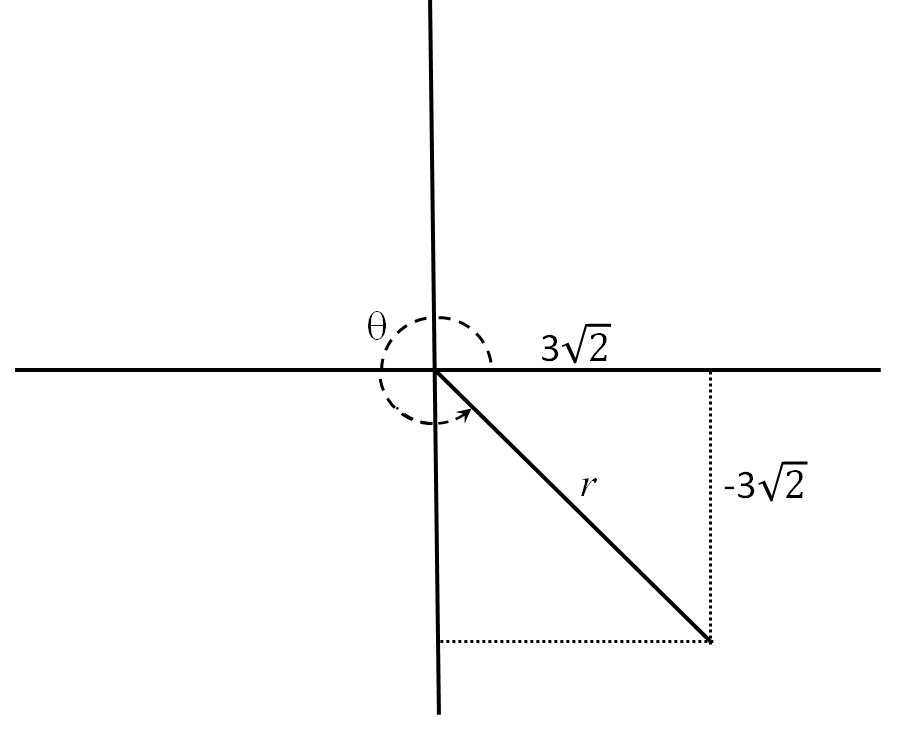
\includegraphics[width=2.5in]
	         {images/polar_to_cart.png}}
	  \caption{\label{fig:complex:polar_to_cart} Modulus and argument of  $z=3\sqrt{2}-3\sqrt{2}\, i$}
\end{figure}

\begin{exercise}{21}
Convert the following complex numbers to rectangular form (that is, write as $a + bi$). Give \emph{exact} answers and not decimals (use square roots if necessary).
\begin{multicols}{2}
\begin{enumerate}[(a)]

\item
$2 \cis(\pi / 6 )$
\item
$5 \cis(9\pi/4)$
\item
$3 \cis(\pi)$
 \item
$\dfrac{\cis(7\pi/4)}{2}$
\item
$\sqrt{2} \cis(5\pi / 3 )$
\item
$\frac{1}{\sqrt{7}} \cis(-7\pi / 6 )$
\item
$14 \cis(30 \pi / 12 )$

\end{enumerate}
\end{multicols}
\end{exercise}

\begin{exercise}{22}
Convert the following complex numbers to polar representation (Give exact answers, no decimal approximations).
\begin{multicols}{3}
\begin{enumerate}[(a)]
 
 \item
$1-i$
\item
$-1 + i$
 \item
$-5$
 \item
$2+2i$
\item
$-2 - 2i$
\item
$\sqrt{3} + i$
 \item
$-3i$
 \item
$2i + 2 \sqrt{3}$
\item
$\sqrt{6} - \sqrt{6}i$
\item
$-3\sqrt{2} - \sqrt{6}i$
\item
$-\sqrt{50} - \sqrt{50}i$
  
\end{enumerate}
\end{multicols}
\end{exercise}

%%% Amplify this exercise
Pictures are essential for gaining an intuitive grasp of how complex numbers work. They're also a lot more fun to draw than mathematical symbols. 

\begin{exercise}{cos form2}
\begin{enumerate}[(a)]
\item
Figure~\ref{polarcoord} shows  polar and Cartesian representations of a complex number $z$  in the complex plane.  Redraw the figure, and put $\overline{z}$ in the picture as well. Show the Cartesian coordinates of $\overline{z}$, as well as the modulus and the complex argument (angle).
\item
Use your picture to obtain the polar representation of $\bar{z}$ in terms of the modulus and complex argument of $z$.
\end{enumerate}
\end{exercise}



The close interrelationship between plane geometry and complex numbers is a rich source of mathematical insight.  The following exercise explores some aspects of this relationship. 

\begin{exercise}{23}
\begin{enumerate}[(a)]
\item
Consider the following set of complex numbers:
\[ \{z \text{ such that } |z| < 2. \} \]
In the complex plane, what does this set look like? Draw a picture, and describe verbally.
\item
Use complex numbers to specify the set of all points on a circle of radius 5 with center at the origin (your answer should look like the set specification given in part (a)).
\item
Consider the following set of complex numbers:
\[ \{z \text{ such that } |z-i| = 2. \} \]
In the complex plane, what does this set look like? Draw a picture, and describe verbally.
\item
Describe the following as a set of complex numbers:  the set of all points on a circle of radius 3 that passes through the origin and has center on the positive $x$-axis.
\end{enumerate}
\end{exercise}

\subsection{Multiplication and powers in complex polar form}

The polar representation of a complex number makes it easy to find
products, quotients, and powers of complex numbers. 

\begin{prop}{polar_mult} Let $z=r\cis\theta$ and $w=s\cis\phi$
be two nonzero complex numbers. Then 
\[z \cdot w=rs\cis(\theta+\phi).\]
Alternatively, we may write
\[r \cis \theta \cdot s \cis \phi =rs\cis(\theta+\phi).\]
 \end{prop}

\begin{proof}
The proof uses the following trigonometric formulas (surely you remember them!):
\newline
\begin{align*}
 \cos(\theta + \phi ) &= \cos\theta\cos\phi - \sin\theta\sin\phi \\
 \sin(\theta + \phi ) &= \cos\theta \cdot \sin\phi + \sin\theta \cdot \cos\phi \\
\end{align*}
\begin{exercise}{24} Fill in the blanks to complete the proof:
\begin{align*}
z \cdot w &= r\cis\theta \cdot \underline{~<1>~} \\
 &= r \left( \cos\theta + i \sin(\underline{~<2>~}) \right) \cdot s  \left( \underline{~<3>~} \right) \\
 &=  rs \cdot \left( \cos\theta + i \sin(\underline{~<4>~}) \right) \cdot  \left( \underline{~<5>~}\right) \\
 &=  rs \left( (\cos\theta \cos\phi   - \sin\theta \sin\phi)  + i(\underline{~<6>~}) \right)\\
 &=  rs  \left( \cos(\theta + \phi) + i\sin( \underline{~<7>~}) \right) \\
 &=  r s  \cis( \underline{~<8>~}) \\
\end{align*}
\end{exercise}
\end{proof}

\begin{exercise}{proof_of_mod2}
Use Proposition~\ref{proposition:complex:polar_mult} and the polar expression for $\bar{z}$ that was given in Section~\ref{subsec:convertRecPolar} to give a simple proof of the following identity:
\[ z \bar{z} = |z|^2. \]
\end{exercise}

We will also want to divide complex numbers in polar form. But first, we need to characterize multiplicative inverses. Note for example that $\left[2 \cis (3\pi / 4)\right]^{-1} = (1/2) \cis (-3 \pi/4)$ since
\[ 2 \cis (3\pi / 4) \cdot (1/2) \cis (-3 \pi/4) = 2 \cdot (1/2) \cdot \cis( 3\pi/4 -3 \pi /4) = \cis(0) = 1, \]
and similarly
\[ (1/2) \cis (-3 \pi/4) \cdot 2 \cis (3\pi / 4)  = \cis(0) = 1. \]

\begin{exercise}{polar_z_inv}
\begin{enumerate}[(a)]
\item
Let $z = 13 \cis\left(\frac{5\pi}{7}\right).$ Find a complex number $w$ (in complex polar form) such that $zw = wz = 1$. Write $w$ so that its argument is between $0$ and $2\pi$. What is the sum of the arguments of $z$ and $w$?
\item
Let $z = \frac{3}{8} \cis\left(0.39\pi\right).$ Find a complex number $w$ (in complex polar form) such that $zw = wz = 1$. Write $w$ so that its argument is between $0$ and $2\pi$. What is the sum of the arguments of $z$ and $w$?
\item
Given that $z=r\cis\theta$ and $w=s\cis\phi$.  Determine what $s$ and $\phi$ must be so that $w = z^{-1}$.  That is, find a value for $s$ and $\phi$ so that 
\[ z \cdot s\cis\phi = s\cis\phi \cdot z = 1.\]
Specify $\phi$ in such a way that it lies in the interval $[0,2\pi]$.
\end{enumerate}
\end{exercise}


\medskip{}
\noindent
From Exercise~\ref{exercise:complex:polar_z_inv} we may deduce that the inverse of a complex number $w = s \cis \phi$ is
\[ w^{-1} = \frac{1}{s}\cis(2\pi -\phi), \]
which we could also write as
\[ w^{-1} = \frac{1}{s}\cis(-\phi) \]
since changing the argument by $2\pi$ does not change the value of the number.

Now recall that to divide two complex numbers $z$ and $w$, we rewrite $\frac{z}{w}$ as $z \cdot w^{-1}$.  
So with $z=r\cis\theta$ and $w=s\cis\phi$ we may divide as follows:  
%Therefore by Proposition~\ref{proposition:complex:polar_mult}, 
\[ \frac{z}{w} = (r\cis\theta) \cdot (\frac{1}{s}\cis(-\phi)) = \frac{r}{s}\cis(\theta - \phi). \]
The previous discussion proves the following proposition.

\begin{prop}{polar_div}
Let $z=r\cis\theta$ and $w=s\cis\phi$ be two nonzero complex numbers. Then
 \[ \frac{z}{w} = \frac{r}{s}\cis(\theta - \phi).\]
 Alternatively, we may write
 \[ \frac{r \cis \theta}{s \cis \phi} = \frac{r}{s}\cis(\theta - \phi).\]
 \end{prop}

\noindent
In summary, multiplication and division of complex numbers in polar form proceeds as follows:

\medskip{}
\noindent
Multiplication:
\begin{itemize}
\item
Multiply the two moduli together to get the modulus of the product.
\item
Add the two arguments together to get the argument of the product.
\end{itemize}

\medskip{}
\noindent
Division:
\begin{itemize}
\item
Divide the modulus of the numerator by the modulus of the denominator to get the modulus of the quotient.
\item
Subtract the argument of the denominator from the argument of the numerator to get the argument of the quotient.
\end{itemize}

\begin{example}{polarmult} If $z=3\cis(\pi/3)$ and $w=2\cis(\pi/6)$,
then $$zw=(2\cdot3)\cis(\pi/3 + \pi/6)= 6 \cis(\pi/2)=6i.$$ \end{example}

\begin{exercise}{25}
Calculate each of the following products using complex polar arithmetic. Give the answer in rectangular form if you can do so without using roots or decimals. Otherwise, leave the answer in polar form.
\begin{enumerate}[(a)]
 
 \item
$2\cis\left(\frac{\pi}{4}\right) \cdot \frac{1}{2} \cis\left( \frac{3\pi}{4}\right)$
 \item
$14\cis\left( \frac{6\pi}{5}\right) \cdot \frac{1}{7} \cis\left( \frac{4\pi}{5} \right) $
\item
$\cis\left(\frac{9\pi}{7}\right) \cdot 2 \cis\left( \frac{8\pi}{7}\right) \cdot 3 \cis\left( \frac{4\pi}{7}\right)$
\item
$\sqrt{3}\cis\left(\frac{\pi}{12}\right)\cdot \sqrt{56}\cis\left(\frac{\pi}{15}\right)\cdot \sqrt{21}\cis\left(\frac{\pi}{15}\right)$
\item
$\sqrt{5}\cis\left(\frac{\pi}{19}\right)\cdot 3^{1/3} \cis\left(\frac{\pi}{3}\right)\cdot 45^{1/3}\cis\left(\frac{-10\pi}{57}\right)$
\end{enumerate}
\end{exercise}

\begin{exercise}{26}
Calculate each of the following quotients using complex polar arithmetic. Give the answers in polar form.
\begin{multicols}{2}
\begin{enumerate}[(a)]
\item
$\dfrac{5\cis\left( \frac{5\pi}{6}\right)}{2\cis \left( \frac{\pi}{2}\right)}$
\item
$\dfrac{27\cis\left(\frac{7\pi}{12}\right)}{6\cis\left(\frac{5\pi}{3}\right)}$
\item
$\dfrac{2\sqrt{2} + 2\sqrt{2}i}{\frac{\sqrt{3}}{4} + \frac{1}{4}i}$
\item
$\dfrac{3 - 3i}{2 - \sqrt{12}i}$
\item
$\dfrac{\sqrt{27} i}{\sqrt{3} - 3i}$
\item
$\dfrac{\sqrt{17} - \sqrt{51} i}{-17 - 17i}$
 
\end{enumerate}
\end{multicols}
\end{exercise}

\noindent
Proposition~\ref{proposition:complex:polar_mult} is the key fact used in finding the following formula for powers of complex numbers in polar form:

\begin{prop}{DeMoivre}(\term{de Moivre's Theorem}) 

Let $z=r\cis\theta$ be a nonzero complex number. Then for $n=1,2,\ldots$ we have
\[ (r\cis\theta)^{n}=r^{n}\cis(n\theta).\tag{$P(n)$}\]
 \end{prop}
(We identify this statement as ``$P(n)$'' for later convenience.)

 Before giving the proof, we first give some general explanation of the ideas behind the proof.
\bigskip
\newline
\noindent {\bf Ideas Behind the Proof}:  We will use a very common proof technique called \term{induction}\index{Induction}.
\footnote{In the Appendix we give a more thorough treatment of the topic of induction. Here we give only a brief presentation.}
 Induction is commonly used to prove statements of the form ``$P(n)$ is true for $n = 1,2,3,\ldots$'', where $n$ is some equation or statement involving the quantity $n$. 

Notice that we actually want to prove an \emph{infinite} number of statements: that is, we want to prove:
\begin{itemize}
\item 
$(r\cis\theta)^{1}=r^{1}\cis\theta$
\item
$(r\cis\theta)^{2}=r^{2}\cis(2\theta)$
\item
$(r\cis\theta)^{3}=r^{3}\cis(3\theta)$
\ldots
\end{itemize}

\noindent The first statement is obviously true. The second statement (for $n=2$) can be proved using Proposition
\ref{proposition:complex:polar_mult}:

\begin{exercise}{27} Prove $(r\cis\theta)^{2}=r^{2}\cis(2\theta)$ using Proposition
\ref{proposition:complex:polar_mult}.
\end{exercise}

The third statement (for $n=3$) can be proved using the statement for $n=2$:

\begin{exercise}{28} Fill in the blanks to complete the proof:
\begin{align*}
(r\cis\theta)^{3} &= r\cis\theta \cdot (\underline{~<1>~})^{2} & \text{(associative)} \\
 &=  r\cis\theta \cdot (r^{2} \cdot\underline{~<2>~}) & \text{(by the previous exercise)}\\
 &=  r^{3} \cdot \cis( \theta +  \underline{~<3>~})) & \mbox{(by Proposition \ref{proposition:complex:polar_mult})}\\
 &=   \underline{~<4>~}) & \mbox{(by basic algebra)}\\
\end{align*}
\end{exercise}

\noindent So we have actually used the statement for $n=2$ to prove the statement for $n=3$. We could continue in this fashion to prove $n=4$ from $n=3$:

\begin{exercise}{29} Prove $(r\cis\theta)^{4}=r^{4}\cis(4\theta)$, using Proposition
\ref{proposition:complex:polar_mult} and the result of the previous exercise 
\hyperref[sec:complex:hints]{(*Hint*)}
\end{exercise}

 \noindent Obviously it would take a long time to prove $n=5$ from $n=4$, $n=6$ from $n=5$, and so on. So instead, we will prove the following statement that covers all these cases:

\[ \text{If } (r\cis\theta)^{k}=r^{k}\cis(k\theta) \mbox{ is true, then } (r\cis\theta)^{k+1}=r^{k+1}\cis((k+1)\theta) \mbox{ is also true.} \]

This allows us to ``ladder up'': if the statement is true for some integer, then it's also true for the {\it next} integer.

In summary, the induction proof has two basic elements:
\begin{itemize}
\item
Prove the statement $P(n)$ for $n=1$ (this is called the ``base case'');
\item
Assuming that $P(n)$  is true for $n=k$, it follows that $P(n)$  is also true for for $n=k+1$ (this is called the ``induction step'').
\end{itemize}

\noindent Now that we've given the ideas, here is the actual proof  of Proposition \ref{proposition:complex:DeMoivre}:
\medskip{}
\newline
\begin{proof}
We will use induction  on $n$. First, for $n=1$ the proposition
is trivial. This establishes the ``base case''. 

Next, assume that $P(n)$ is true for $n=k$: that is, 
$z^k = r^k \cis(k \theta)$. Then using this fact and exponent rules, we may rewrite $z^{k+1}$ as
\begin{align*}
z^{k+1} & =z^{k}z\\
 & =r^{k}\cis(k\theta)\,r(\cis\theta)\\
 & =r^{k+1}[\cis(k\theta + \theta)]\\
 & =r^{k+1} \cis[(k+1)\theta].
\end{align*}
This establishes the ``induction step'', which completes the proof.
\end{proof}

\begin{example}{DeMoivre} We will compute $z^{10}$ where $z=1+i$. Rather than computing $(1+i)^{10}$ directly, it
is much easier to switch to polar coordinates and calculate $z^{10}$
using de Moivre's Theorem: \begin{align*}
z^{10} & =(1+i)^{10}\\
 & =\left(\sqrt{2}\cis\left(\frac{\pi}{4}\right)\right)^{10}\\
 & =(\sqrt{2}\,)^{10}\cis\left(\frac{5\pi}{2}\right)\\
 & =32\cis\left(\frac{\pi}{2}\right)\\
 & =32i.\end{align*}
 \end{example}
 
\noindent
Notice that de Moivre's Theorem says nothing about a complex number raised to negative powers.  For any real number $x$, we know $x^{-n}$ means $(x^n)^{-1}$.  Complex numbers happen to work the same way.
 
 \begin{defn} \label{polar_negpower}
 Given a complex number $z=r\cis\theta$, 
 \[ z^{-n} = (z^n)^{-1}. \]
 \end{defn}
 
 \begin{example}{5}
Let $z = 2\cis(\pi/4)$.  What is $z^{-3}$?  
 \begin{align*}
  z^{-3} & = (z^3)^{-1} \\
  & = ([2\cis(\pi/4)]^3)^{-1} \\
  & = (8\cis(3\pi/4))^{-1} \quad \mbox{ (by de Moivre's Theorem) } \\
  & = \frac{1}{8}\cis(5\pi/4) \qquad \mbox{ (by Exercise~\ref{exercise:complex:polar_z_inv}) } 
  \end{align*}
  \end{example}
 
 

\begin{exercise}{31}
Calculate each of the following expressions. Write the answer as $a + bi$ if you can do so without using roots or decimals. Otherwise, you may leave the answer in polar form.
\begin{multicols}{2}
\begin{enumerate}[(a)]
 
 \item
$(1+i)^{-3}$
 \item
$(1 - i)^{6}$
 \item
$(\sqrt{3}+i)^{5}$
 \item
$(-i)^{10}$
 \item
$((1-i)/2)^{4}$
 \item
$(-\sqrt{2} - \sqrt{2}\, i)^{12}$
 \item
$(-2+2i)^{-5}$
\item
$(\sqrt{2 + \sqrt{2}} - i\sqrt{2 - \sqrt{2}})^{16}$
\item 
$\frac{(\sqrt{15} -3 \sqrt{5}i)^5}{60^2}$
\item
$\frac{(1-i)^{10}}{(-\sqrt{3} + i)^6}$
\end{enumerate}
\end{multicols}
\end{exercise}


\subsection{A Remark on representations of complex numbers}\label{remRepComplex}

We have seen that a complex number \emph{z} can be expressed in a
number of different ways: 
\begin{itemize}
\item As $a+bi$, where $a$ and $b$ are real numbers; 
\item As a point in the Cartesian (two-dimensional) plane; 
\item As a pair of real numbers ($a,b$) that give the rectangular coordinates
of the point in the plane; 
\item As a pair of numbers $(r,\theta)$ where $r\geq0$ and $0\le\theta<2\pi$,
that give the polar coordinates of the point in the plane; 
\item As $r\cdot(\cos\theta+i\cdot\sin\theta)$, or the equivalent form
$r\cdot\cis(\theta)$.
\end{itemize}
In abstract mathematics, it is very common to represent the ``same''
entity in a number of different ways. One of the main goals of abstract
algebra is to identify mathematical structures that are the ``same''
algebraically even though they appear to be different. Mathematical
structures that are the ``same'' algebraically are said to be
\term{isomorphic}. We will be seeing isomorphic structures
throughout this course.

The importance of isomorphism in mathematics cannot be overstated.\footnote{There are other types of ``morphisms'' as well, such as homeomorphism (in topology), diffeomorphism (in differential topology), and just plain morphism (in category theory).}  Realizing that the same thing can be represented in two different ways is often the key to mathematical progress, and can lead to enormous simplifications. For instance, we have seen that it's  easier to add complex numbers in Cartesian form, while it's much simpler to multiply complex numbers in polar form.  Since Cartesian and polar forms  are simply two different ways of representing the same thing, we can freely switch back and forth between the two forms, using whichever is most convenient at the moment. 

\begin{exercise}{cos form}
\begin{enumerate}[(a)]
 \item
Using de Moivre's formula for $z^3$ where $z =  \cis \theta$, find formulas for $\cos 3 \theta$ and $\sin 3 \theta$ in terms of $\cos \theta$ and $\sin \theta$. \hyperref[sec:complex:hints]{(*Hint*)}
\item
Using part (a), find a formula for $\cos 3 \theta$ in terms of $\cos \theta$.  
\hyperref[sec:complex:hints]{(*Hint*)}
\item
Show that for any $n$, it is always possible to find a formula for $\cos n\theta$ in terms of $\cos \theta$.
\item
* Show that for any \emph{even} $n$, it is always possible to find a formula for $\cos n\theta$ in terms of \emph{even} powers of $\cos \theta$.
\end{enumerate}
\end{exercise}


\section{Complex numbers and roots of algebraic equations}
\label{sec:complex_roots}

\subsection{Roots of unity and regular polygons\quad\sectionvideohref{c5WbBwp5av4&index=6&list=PL2uooHqQ6T7PW5na4EX8rQX2WvBBdM8Qo}}\label{sec:RootsOfUnity}
As we mentioned before, complex numbers got their start when mathematicians started considering the solutions to algebraic  equations. One particularly important equation is
\[z^{n}=1, \qquad \text{ where } n \in \mathbb{N}.\]
For example, when $n=4$ the complex numbers which solve $z^4=1$ are $z=1$, $-1$, $i$, and $-i$. In general, the complex numbers that satisfy the
equation $z^{n}=1$ are called the \term*{$n$th roots of unity}\index{Roots! of unity}. (In other words, ``$n$th root of unity'' means the same thing as ''$n$th root of 1''.)

\begin{exercise}{48}
\begin{enumerate}[(a)]
\item
Give two distinct square roots of unity (that is, $z^n = 1$ for $n=2$).
\item
For what integers $n$ is $-1$ an $n$th root of unity?
\end{enumerate}
\end{exercise}

It turns out that in general we can find $n$ different $n$th roots of unity, as per the following proposition:

\begin{prop}{nth_roots_of_1}The complex number $z$ is an $n$th root of unity if and only if $z$ satisfies the following condition:
\[
z=\cis\left(\frac{2k\pi}{n}\right), \text{ where } k \text{ is an integer between }0 \text{ and } n-1.\] 
\end{prop}

To illustrate this proposition, consider the case $n=4$. Then the equation gives: $z=\cis(2k\pi/4)$  where $k=0,1,2,3$, which works out to $\cis(0)$, $\cis(\pi/2)$, $\cis(\pi)$, and $\cis(3\pi/2)$.  Converting to Cartesian form we get  $1, i , -1, -i$ as our four roots, in perfect agreement with what we found in the first paragraph of this section.

So, let's give a proof!

\begin{proof}
The proposition is an ``if and only if'' assertion, meaning that we'll have to prove it both ways. We'll start with the ``only if '' part.  To this end, we suppose $z$ is a complex $n$th root of unity. Our  goal is to show that $z$ must satisfy the given formula. Any complex number may be written in polar form, so we may write $z = r \cis(\theta)$ where $r$ is the modulus and $\theta$ is the complex argument of $z$.  So we may deduce:
\begin{align*}
z^n &= 1 & (z \text{ is a } n\text{th root of unity})\\
\implies &(r \cis(\theta))^n=1 & (\text{polar form of } z)\\
\implies &r^n \cis(n\theta)=1 & (\text{de Moivre's theorem})\\
\implies &|r^n \cis(n\theta)|=|1| & (\text{take modulus of both sides})\\
\implies &|r|^n =1 & (\text{properties of modulus})\\
\implies &r =1. & (\text{Since }r\text{ is a nonnegative number})\\
\end{align*}

\noindent
Now substituting $r=1$ back into the third line in this series of implications, we get:

\begin{align*}
\cis(n\theta)&=1 & (\text{substitution})\\
\implies &\cos(n\theta) + i\sin(n\theta) =1 & (\text{definition of cis})\\
\implies &\cos(n\theta)=1 \text{ and } \sin(n\theta)=0 &(\text{equality of complex numbers})\\
\implies &n\theta = m \cdot 2\pi &\text{(periodicity of sin and cosine, from trig)}\\
\implies &\theta = m\cdot 2\pi/n. &\text{(basic algebra)}
\end{align*}

\noindent
To recap, we have:
\[z= r \cis(\theta) \text{ where } r=1 \text{ and } \theta = 2\pi m/n, \text{ where }m \text{ is an integer}.\]

Now, any fraction of the form $m/n$ can be written as an integer plus a fractional part between 0 and 1. Furthermore, the fractional part always has the form $k/n$ where $k$ is an integer between 0 and $n-1$. In other words:
\[m/n  = \ell + k/n \qquad \text{where } \ell \text{ and } k \text{ are integers and } 0 \le k < n.\]
It follows by substitution that
\begin{align*}
z= &\cis(2\pi m/n)&\text{(from last equality in previous series)}\\
& \implies z= \cis(2\pi (\ell + k/n))&\text{(substitution)}\\
& \implies z= \cis(2\pi\ell) \cis(2\pi k/n)&\text{(algebraic properties of cis)}\\
& \implies z=  \cis(2\pi k/n).&\text{(def.  of cis and trig)}\\
\end{align*}

Our goal has been achieved: $z$ must definitely have the form $\cis(2\pi k/n)$ where $0 \le k < n$.

Now for the ``if'' part; we must show that complex numbers which satisfy the formula as also $n$th roots of unity.  By de Moivre's Theorem, 
\[ z^{n}=\cis\left(n\frac{2k\pi}{n}\right)=\cis(2k\pi)=1.\]
Finished!

\end{proof}

\begin{rem}
Note that the condition
\[
z=\cis\left(\frac{2k\pi}{n}\right), \text{ where } k \text{ is an integer between }0 \text{ and } n-1.\] 
does indeed specify $n$ distinct values for $z$.  This is because $k/n$ produces $n$ different fractions between 0 and 1, so $\frac{2k\pi}{n}$ gives $n$ different angles between 0 and $2\pi$. Our vector representation of complex numbers tells us that different angles must produce different complex numbers.
\end{rem}

\begin{exercise}{49}
\begin{enumerate}[(a)]
\item
Using Proposition~\ref{proposition:complex:nth_roots_of_1}, write three cube roots of unity in polar form. Convert to the form $a + bi$.
\item
Using Proposition~\ref{proposition:complex:nth_roots_of_1}, write six 6th roots of unity in polar form. Convert to the form $a+bi$.
\end{enumerate}
\end{exercise}

\begin{exercise}{50}
In this exercise you will give a different proof that there are exactly 4 4th roots of unity, by showing that any complex apart from 1, -1, $i$, or $-i$  cannot possibly be a 4th root of unity. First we suppose that $w$ is a complex number such that $w \notin \{1,-1,i,-i \}$. 
\begin{enumerate}[(a)]
\item
Show that $(w-1)(w+1)(w-i)(w+i) \neq 0$.
\hyperref[sec:complex:hints]{(*Hint*)}
\item
Show that this implies that $w$ is not a 4th root of unity.
\hyperref[sec:complex:hints]{(*Hint*)}
\end{enumerate}
\end{exercise}

\begin{exercise}{51}
\begin{enumerate}[(a)]
\item
Multiply out the product $(z - 1)(z - \cis\left(\frac{2\pi}{3}\right))(z - \cis\left(\frac{4\pi}{3}\right))$ and simplify.
\hyperref[sec:complex:hints]{(*Hint*)}
\item
Use your result in (a) to show that there are exactly 3 cube root of unity. 
\end{enumerate}
\end{exercise}

When represented in the complex plane, the roots of unity have some very interesting geometric properties:

\begin{example}{rootsunity} The 8th roots of unity can be represented
as eight equally spaced points on the unit circle (Figure~\ref{rtsunity}).
For example, some 8th roots of unity are \begin{align*}
\omega & =\frac{\sqrt{2}}{2}+\frac{\sqrt{2}}{2}i\\
\omega^{3} & =-\frac{\sqrt{2}}{2}+\frac{\sqrt{2}}{2}i\\
\omega^{5} & =-\frac{\sqrt{2}}{2}-\frac{\sqrt{2}}{2}i\\
\omega^{7} & =\frac{\sqrt{2}}{2}-\frac{\sqrt{2}}{2}i.\end{align*}
In fact, the 8th roots of unity form a \emph{regular octagon}.
 \end{example}

%
\begin{figure}[hbt]
\begin{center}
\tikzpreface{cyclic_roots_unity}
\begin{tikzpicture}[scale=1.65] %Replaced figure with tikz figure - TWJ 5/6/2010

\draw [->]  (0,-1.5) -- (0,1.5);
\draw  [->] (-1.75,0) -- (1.75,0);
\node [right] at (0,1.5) {$y$};
\node [below] at (1.75,0) {$x$};
\node [below] at (0.1,0) {$0$};

\draw (0,0) circle (1);

\filldraw[fill=black, draw=black] (0:1) circle (0.03);
\filldraw[fill=black, draw=black] (45:1) circle (0.03);
\filldraw[fill=black, draw=black] (90:1) circle (0.03);
\filldraw[fill=black, draw=black] (135:1) circle (0.03);
\filldraw[fill=black, draw=black] (180:1) circle (0.03);
\filldraw[fill=black, draw=black] (225:1) circle (0.03);
\filldraw[fill=black, draw=black] (270:1) circle (0.03);
\filldraw[fill=black, draw=black] (315:1) circle (0.03);


\node [right] at (1,-0.15) {1};
\node [right] at (45:1) {$\omega$};
\node [left] at (0,1.15) {$i$};
\node [left] at (135:1) {$\omega^3$};
\node [left] at (-1,-0.15) {$-1$};
\node [left] at (225:1) {$\omega^5$};
\node [left] at (0,-1.15) {$-i$};
\node [right] at (315:1) {$\omega^7$};

\end{tikzpicture}

\end{center}
\caption{8th roots of unity}
\label{rtsunity}
\end{figure}
 
\begin{exercise}{52}
Sketch the cube roots of unity in the complex plane. Use the distance formula (from geometry) to show that the three points are all the same distance from one another.  Connect the three points to form a triangle. What kind of triangle is it?
\end{exercise}

\begin{exercise}{53}
Prove (using geometry) that the 4th roots of unity form a square. (\emph{Hint}: Besides showing that all sides are equal, you also have to show that they are perpendicular.)
\end{exercise}

\begin{exercise}{54}
*Prove (using geometry) that the 6th roots of unity form a regular hexagon. (\emph{Hint}: Draw lines from each point to the origin, forming 6 triangles. What can you say about these triangles?)
\end{exercise}

Once again, we see an interesting relationship between complex numbers and plane geometry.  Let us explore this relationship a little further.

\begin{exercise}{hexagon_rotate}
\begin{enumerate}[(a)]
\item
Draw a picture of the  6th roots of unity in the complex plane. Label them $A,B,C,D,E,F$ with $A=1, B= \cis\left(\frac{2\pi}{6}\right),$ and $C,D,E,F$ going counterclockwise around the circle.
\item
Fill in each of the following blanks with the letter corresponding to the product of the two complex numbers. For example,  $B \cdot B = \cis\left(\frac{2\pi}{6}\right) \cdot \cis\left(\frac{2\pi}{6}\right) = \cis\left(\frac{2\pi}{3}\right) = C$.

\begin{multicols}{3}
$B \cdot A = \underline{~<1>~}$

$B \cdot B = \underline{~<2>~}$ 

$B \cdot C = \underline{~<3>~}$

$B \cdot D = \underline{~<4>~}$

$B \cdot E = \underline{~<5>~}$ 

$B \cdot F = \underline{~<6>~}$
\end{multicols}

\item
Using your answers from part (b), on your picture draw an arrow from $A$ to $B \cdot A$; similarly draw arrows from $B$ to $B \cdot B$, $C$ to $B \cdot C$, and so on. What do you observe about the arrows?
\item
It appears that multiplying all of the corners of the hexagon $ABCDEF$ by $B$ produces a \emph{rotation} of the hexagon. What is the angle of rotation?
\item
Fill in the blanks:
\begin{multicols}{3}
$E \cdot A = \underline{~<1>~}$

 $E \cdot B = \underline{~<2>~}$

 $E \cdot C = \underline{~<3>~}$

$E \cdot D = \underline{~<4>~}$

$E \cdot E = \underline{~<5>~}$

 $E \cdot F = \underline{~<6>~}$.

\end{multicols}

\item Just as in part (c), use your answers from part (d) to draw arrows from $A$ to $E \cdot A$, $B$ to $E \cdot B$, etc. What do you observe about the arrows? 

\item
Fill in the blanks:  If you choose one particular 6th root of unity and multiply it with all the other 6th roots, the new values correspond to different $\underline{~<1>~}$ of the original hexagon. The angle of $\underline{~<2>~}$ is equal to the complex argument of the $\underline{~<3>~}$.
\end{enumerate}
\end{exercise}

\begin{exercise}{55}
\begin{enumerate}[(a)]
\item
Just as in part (b) of Exercise~\ref{exercise:complex:hexagon_rotate} fill in the blanks with the correct letter $A,B,C,D,E$ or $F$ (recall that $\overline{A}$ denotes the complex conjugate of $A$).
\begin{multicols}{3}
$ \overline{A} = \underline{~<1>~} $

$  \overline{B} = \underline{~<2>~}$

$  \overline{C} = \underline{~<3>~}$

 $ \overline{D} = \underline{~<4>~}$

$ \overline{E} = \underline{~<5>~}$

 $ \overline{F} = \underline{~<6>~}).  $
\end{multicols}
\item 
Just as in part (c) of Exercise~\ref{exercise:complex:hexagon_rotate}, draw arrows from $A$ to $\overline{A}$, $B$ to $\overline{B}$, etc. What do you observe about the arrows?

\item We refer to the geometrical motion produced by complex conjugation as ``flipping". What is the axis of the ``flip'' that is produced by taking the complex conjugates of the sixth roots of unity?
\end{enumerate}
\end{exercise}

The previous exercises (when suitably generalized) lead to the following stupendous conclusion:

\begin{itemize}
\item
Every \emph{rigid} motion of a regular $n$-gon is equivalent to some combination of complex conjugation and multiplication by one of the $n$th roots of unity. (By ``rigid motion'' we mean any motion that a rigid object could undergo, without stretching or bending or distorting it in any way. We'll have more to say about rigid motions in Chapter~\ref{symmetries}.) 
\end{itemize}

\begin{exercise}{non_comm}
\begin{enumerate}[(a)]
\item 
What geometrical motion corresponds to the following algebraic operation:
Multiply all 6th roots by $D$, then take the complex conjugates.

\item 
What geometrical motion corresponds to the following algebraic operation:
``Take the complex conjugates of all 6th roots, then multiply by  $D$.''

\item 
What geometrical motion corresponds to the following algebraic operation:
``Multiply all 6th roots by $C$, then take the complex conjugates.''

\item 
What geometrical motion corresponds to the following algebraic operation:
``Take the complex conjugates of all 6th roots, then multiply by  $C$.''

\end{enumerate}
\end{exercise}

Exercise~\ref{exercise:complex:non_comm} also gives us our first exposure to a phenomenon that is quite common in abstract algebra, namely the existence of non-commutative operations (also known as \term*{non-abelian}\index{operations!non-abelian}\index{non-abelian operations} operations).
 We saw that both multiplication by a $n$th root of unity and complex conjugation corresponded to motions of a regular $n$-gon. However, the \emph{order} of the motions matters: rotating first and then conjugating (i.e. ``flipping'') gives a \emph{different} result than conjugating first, then performing the rotation afterwards.

\begin{exercise}{56}
If you've studied matrix multiplication, then you may have seen non-commutative operations before: 
\begin{enumerate}[(a)]
\item
Give an example of two $2\times2$ matrices that do \emph{not} commute: that is $AB \neq BA$.
\item
Give an example of two $2\times2$ matrices that \emph{do} commute.
\end{enumerate}
\end{exercise}

The previous exercises give a small hint as to the extensive and beautiful relationship between the complex numbers and plane geometry.  The following exercises further explore  this relationship.  (\emph{Hint}: you may find that complex polar form is useful in these exercises.)

\begin{exercise}{57}
Consider a plane with Cartesian coordinates. Let $O$ be the point $(0,0)$, let $A$ be the point $(a,b)$, and let $C$ be the point $(c,d)$. Also, let $z = a+bi$ and $w = c+di$.
\begin{enumerate}[(a)]
\item
*  Show that 
\[
\text{Area of triangle }OAC = \left| \frac{z \bar{w} - \bar{z} w}{4} \right|. \]
\item
* Show that $\overline{OA}$ is perpendicular to $\overline{OC}$ if and only if $z \bar{w} + \bar{z} w = 0$.
\item
* Use complex arithmetic to prove the \emph{Law of cosines}\index{Law of cosines}:
\[ AC^2 = OA^2 + OC^2 - 2(OA)(OC)\cos(\angle AOC),\]
where $AC,OA$, and $OC$ denote the lengths of segments $\overline{AC}, \overline{OA}$ and $\overline{OC}$ respectively. 
\hyperref[sec:complex:hints]{(*Hint*)}

\end{enumerate}
\end{exercise}

In fact, many intricate theorems in plane geometry that require long proofs using conventional methods can be proven much more easily using complex numbers. We will not be exploring this further; but we hope these examples will stimulate your imagination!


\subsection{Complex $n$th roots in general 
\quad\sectionvideohref{o5wpaYsDU4o&list=PL2uooHqQ6T7PW5na4EX8rQX2WvBBdM8Qo&index=7}}\label{rootsingeneral}

In the previous section, we characterized all complex solutions of the equation $z^n = 1$; we called these solutions the $n$th roots of unity. A natural question to ask then is, What about the $n$th roots of any complex number? That is, given a complex number $a + bi$, can we find all solutions to the equation $z^n = a + bi$? Let's explore some simple cases first.

\begin{exercise}{58}
\begin{enumerate}[(a)]
\item
Find all square roots of 1. 
\item
Find all square roots of 4.
\item
Find all square roots of -1.
\item
Find all square roots of -2.
\item
In each of the above cases, given one of the square roots, you can find a second square root by multiplying by \underline{~~~~~} (fill in the blank).
\end{enumerate}
\end{exercise}
We may use the observation from part (e) of the previous exercise to find find alternative square roots of other complex numbers.

\begin{exercise}{58a}
\begin{enumerate}[(a)]
\item
 The complex number $1 + i$ is one square root of $2i$. Can you find another one?
\item
Find two square roots of $8i$.
\hyperref[sec:complex:hints]{(*Hint*)}
\item
Find two square roots of $-8i$.
\end{enumerate}
\end{exercise}

Next, let us consider the case of cube roots. Consider for example the cube roots of $1 + i$, which are the solutions to
\[ z^3 = 1 + i. \]
We  may rewrite this in polar form as
\[ (r \cis \theta)^3 = \sqrt{2} \cis\left(\frac{\pi}{4}\right), \]
where $r \cis \theta$ is $z$ in polar form. De Moivre's theorem then gives us:
\[ r^3 \cis 3\theta = \sqrt{2} \cis\left(\frac{\pi}{4}\right). \]
One solution for $r$ and $\theta$ which satisfies this equation is:
\[ r^3 = \sqrt{2} \implies r=2^{1/6} \quad \textrm{ and } \quad 3\theta = \pi/4 \implies \theta = \pi/12, \]
so that
\begin{align*}
z &=  2^{1/6} \cis(\pi/12).
\end{align*}
We may use deMoivre's theorem to verify that this $z$ is indeed a cube root of $1+i$.  But is it the only one?
 In fact, if we multiply this $z$ by $\cis(2 \pi/3)$ and cube the result, we find:
\begin{align*}
 \left( 2^{1/6} \cis(\pi/12) \cdot \cis(2\pi/3) \right)^3 &= \left( 2^{1/6} \cis(\pi/12) \right)^3 \cdot \left(\cis(2\pi/3) \right)^3 \\
&= (1+i) \cdot 1 \\
&= 1+i,
\end{align*}
so that $z \cdot \cis(2\pi/3)$ is also a cube root of $1+i$.  Why does this work? Notice that $\cis(2\pi/3)$ is a \emph{cube root of unity}, so it turns into 1 when cubed. The same thing happens with $\cis(4\pi/3)$, which is the other cube root of unity--you may check that $z \cdot \cis(4\pi/3)$ is an additional cube root of $1+i$.
This example suggests a general procedure for finding $3$ distinct cube roots of complex numbers:
\begin{itemize}
\item Find a single cube root using de Moivre's Theorem;
\item Multiply your result by $ \cis(2\pi/3)$  and $ \cis(4\pi/3)$ to obtain $3$ distinct cube roots.
\end{itemize}

This takes care of cube roots. But let's not stop there! We can use a similar procedure to find  $n$ distinct $n$th roots of any complex number:
\begin{itemize}
\item Find a single root using de Moivre's Theorem;
\item Multiply your result by all $n$ roots of unity to obtain $n$ distinct roots.
\end{itemize}

\begin{exercise}{59}
Show that the 2-step procedure above gives \emph{all} $n$th roots of a given complex number. That is, show that any complex $n$th root of $z$ can be obtained as an $n$th root of unity times any other complex $n$th root of $z$. You may proceed as follows. Suppose $z$ is a complex number, and $w_1$ and $w_2$ are $n$th roots of $z$. Show that there exists an $n$th root of unity $u$ such that $w_1$ is the product of $u$ and $w_2$, i.e. $w_1=u \cdot w_2$. 
\end{exercise}

\begin{exercise}{60}
(In this exercise, you may leave your answers in polar form)
\begin{enumerate}[(a)]
\item
Find all fifth roots of $-i$.
\item
Find all fourth roots of $-1 + \sqrt{3}i$.
\item
Find all fourth roots of $ \sqrt{1/2 + \sqrt{2}/4} + i\sqrt{1/2 - \sqrt{2}/4}$. 
\hyperref[sec:complex:hints]{(*Hint*)}
\item
Find all sixth roots of $-16i$.
\item
Find all seventh roots of $5 - 5i$.
\end{enumerate}
\end{exercise}

\begin{exercise}{60a}
In previous exercises, we have considered $n$th roots where $n$ is a \emph{positive} integer. But what about \emph{negative} roots?
\begin{enumerate}[(a)]
\item
For parts (a-d) in Exercise~\ref{exercise:complex:60}, find the corresponding \emph{negative} roots (i.e., in part (a) find the negative 5th roots, etc).
\item
Explain the relationship between the moduluses of the roots you found in Exercise~\ref{exercise:complex:60}, and the roots you found in part (a).
\item
Explain the relationship between the complex arguments of the roots you found in Exercise~\ref{exercise:complex:60}, and the complex arguments you found in part (a).
\end{enumerate}
\end{exercise}

\subsection{Complex roots of polynomial equations\quad
\sectionvideohref{HKtljwos03o&index=8&list=PL2uooHqQ6T7PW5na4EX8rQX2WvBBdM8Qo}}\label{sec:FTOA}

Next we consider more general algebraic equations than the basic $n$th root equations we've been looking at so far.\index{Roots! of polynomial equations}  As a first example, consider the equation $z^2 + pz = q$, where $p$ and  $q$ are real numbers. Using  the quadratic formula, it is not too hard to show that if $a + bi$ is a solution of $z^2 + pz = q$ then the complex conjugate $a - bi$ is also a solution. This is because  $z^2 + pz = q$ can also be written as  $z^2 + pz - q = 0$, and the quadratic formula tells us that there are two solutions, given by:
$$ z = \frac{-p \pm \sqrt{p^2 - (4)(1)(-q)}}{2} = \frac{-p}{2}  \pm \frac{\sqrt{p^2 + 4q}}{2}.$$
The $-p/2$ term is always real, but the square root term is either real or imaginary depending on the sign of $p^2 + 4q$  (since $q$ could be negative).  If the square root term is real, then both roots are real, and each root is its own complex conjugate.  If the square root term is imaginary, then the $\pm$ means that the imaginary parts of the two roots are negatives of each other, so that the two roots are complex conjugates.

\begin{exercise}{cubic_conj}
Consider the cubic equation $z^3 + pz^2 + qz = r$, where $p, q$ and  $r$ are all real numbers.
\begin{enumerate}[(a)]
\item
Using an appropriate identity from Exercise \ref{exercise:complex:cxprops}, show that $\overline{z^3} = \overline{z}^3$.
\item
Similarly, show  $\overline{pz^2} = p\overline{z}^2$ and $\overline{qz} = q\overline{z}$, and $\overline{r} = r$.
\item 
Use (a) and (b) to show that $\overline{z^3 + pz^2 + qz - r} = \overline{z}^3 + p\overline{z}^2 + q\overline{z} - r$.
\item
Using (c), show that $z^3 + pz^2 + qz - r = 0$ implies that $\overline{z}^3 + p\overline{z}^2 + q\overline{z} - r = 0$.
\item
Using (d), show that if $z$ is a solution to $z^3 + pz^2 + qz = r$ then $\overline{z}$ is also a solution.
\end{enumerate}
\end{exercise}

\begin{exercise}{conjugate_root2a}
Suppose the cubic equation $z^3 + pz^2 + qz = r$ has an odd number of solutions. Show that at least one of the solutions must be real.
\end{exercise}


The proof in Exercise~\ref{exercise:complex:cubic_conj} can be straightforwardly generalized to quartic, quintic, and higher-degree polynomials as well. The result is:

\begin{prop}{nth_degree_conj}   Given that the complex number $z$ is a solution of $z^n + a_{n-1}z^{n-1} + a_{n-2} z^{n-2} + \ldots + a_1 z =a_0,$ where $a_0, a_1, \ldots a_{n-1}$ are real numbers. Then $\overline{z}$ is also a solution to the same equation. 
\end{prop}

\begin{exercise}{62} 
Given that $3 - 7i$ and $-2+i$ are solutions to an equation of the form $z^4 + a_{3}z^{3} + a_{2} z^{2}+ a_1 z + a_0 = 0$ where $a_0, a_1, a_2, a_3$ are real. 
\begin{enumerate}[(a)]
\item
Find two other solutions to the same equation.
\item
*Find $a_0, a_1, a_2, a_3$. 
\hyperref[sec:complex:hints]{(*Hint*)}
\end{enumerate}
\end{exercise}

\begin{exercise}{62a} 
Given that  $p(z) =z^3 +  a_{2} z^{2}+ a_1 z + a_0 = 0$, where $a_0, a_1, a_2$ are real numbers. Suppose $p(1) = 16$, and suppose that $1 + 2i$ is a root of $p(z)$.  
\begin{enumerate}[(a)]
\item
Find two other solutions to the same equation.
\item
Find $a_0, a_1, a_2$. 
\end{enumerate}
\end{exercise}

\begin{exercise}{conjugate_root2}
Given the equation  $z^n + a_{n-1}z^{n-1} + a_{n-2} z^{n-2} + \ldots + a_1 z =a_0,$ where $a_0, a_1, \ldots a_{n-1}$ are real numbers. Let $N$ be the number of solutions of the equation that are \emph{not} real. Prove that either $N=0$ or $N$ is divisible by 2. 
\hyperref[sec:complex:hints]{(*Hint*)}
\end{exercise}

\begin{exercise}{cr2}
Suppose that $p(z)$ is a fourth degree polynomial with real coefficients. Suppose that $p(z) = p(-z)$. Suppose also that $3+4i$ is a root of $p(z)$  and that $p(0) = 1$.  
\begin{enumerate}[(a)]
\item
Find three other roots of $p(z)$.
\item
Find $p(z)$. 
\end{enumerate}
\end{exercise}


The most famous result concerning complex roots of polynomials is known as the {\bf \emph{Fundamental Theorem of Algebra}}:

\begin{prop}{FTOA} Given any equation of the form $z^n + a_{n-1}z^{n-1} + a_{n-2} z^{n-2} + \ldots + a_1 z =a_0,$ where $n>0$ and $a_0, a_1, \ldots a_{n-1}$ are real numbers. Then there exists at least one and at most $n$ distinct complex numbers which solve the given equation. 
\end{prop}

The Fundamental Theorem of Algebra actually has two parts. The easy part is the ``at most $n$ distinct complex roots'' part, and the hard part is the ``at least one complex root'' part. We will eventually prove the easy part in Chapter~\ref{poly}, but sadly the hard part is beyond our scope. For more information on this see the  Remark  at the end of the chapter.

\begin{exercise}{70}
\begin{enumerate}[(a)]
\item
Give an example of an equation of the form $z^2 + a_1z = a_0$ that has only one solution.
\item
Give an example of an equation of the form $z^3 + a_2z^2 + a_1 z = a_0$ that has only one solution.
\item
Can you give an example of an equation of the form $z^3 + a_2z^2 + a_1 z = a_0$ that has exactly two solutions?
\end{enumerate}
\end{exercise}


\begin{exercise}{72}
Using the Fundamental Theorem of Algebra and Exercise~\ref{exercise:complex:conjugate_root2}, prove the following proposition: 
Given an equation of the form $z^n + a_{n-1}z^{n-1} + a_{n-2} z^{n-2} + \ldots + a_1 z =a_0,$ where $n>0$ and $a_0, a_1, \ldots. a_{n-1}$ are real numbers. Suppose the equation has no real solutions. Then the equation has at least two distinct solutions.
\end{exercise}

\begin{exercise}{72a}
Using the Fundamental Theorem of Algebra and Exercise~\ref{exercise:complex:conjugate_root2}, prove the following proposition: 
Given an equation of the form $z^n + a_{n-1}z^{n-1} + a_{n-2} z^{n-2} + \ldots + a_1 z =a_0,$ where $n$ is a positive odd number and $a_0, a_1, \ldots. a_{n-1}$ are real numbers.  Then the equation has at least one real solution.
\end{exercise}


\begin{exercise}{72b}
Give an example of a polynomial of the form  $z^6 + a_{5}z^{5} + a_{4} z^{4} + \ldots + a_1 z =a_0,$ that has no real solutions, and exactly two distinct complex solutions.
\end{exercise}


\begin{rem} (\emph{historical background})
 The Fundamental Theorem of Algebra is a famous ``hard problem'' in the history of mathematics. Some of the greatest mathematicians in history (including Euler, Lagrange, Laplace, and Gauss) thought they had proofs, only to have later mathematicians point out flaws or gaps in the arguments. See \url{http://www-history.mcs.st-and.ac.uk/HistTopics/Fund_theorem_of_algebra.html} for more details. In the modern mathematics curriculum, the proof  is usually given in courses on complex analysis as an easy consequence of ``Liouville's theorem'', which was first proved in 1847. Modern college students who learn basic concepts from the theory of complex variables can readily grasp the theorem which stymied the greatest mathematical minds of history.
\end{rem}

\section{Applications of complex numbers\quad
\sectionvideohref{beo_65G9I7Q&list=PL2uooHqQ6T7PW5na4EX8rQX2WvBBdM8Qo&index=6}}
\label{sec:ApplicationComplexNumbers}

\subsection{General remarks on the usefulness of complex numbers}

We have already discussed that it took some time for complex numbers to be generally accepted by mathematicians, who tended to have a preference for ``pure'' numbers such as the integers. But complex numbers have had their revenge. Today the ``purest'' form of mathematics, namely number theory, is heavily dependent on complex numbers. The famous Fermat's Last Theorem\index{Fermat!last theorem} was proved using techniques that involved complex numbers.\footnote{See \url{http://www-history.mcs.st-and.ac.uk/HistTopics/Fermat's_last_theorem.html} for some of the long and sordid history of Fermat's Last Theorem.}

But quite apart from pure mathematics, complex numbers have proved to be extremely practical. Complex numbers are indispensable tools for
scientists and engineers. Virtually all of modern physics is based
on complex numbers. Engineers build bridges using complex numbers.
Without complex numbers, there would probably be no computers, cell
phones or most other electronics. A strong argument could be made that complex numbers are even more useful than ``real'' numbers.

Much of the practical usefulness of complex numbers comes from their close relationship
with the trigonometric functions cosine and sine. We have seen a little
bit of this already in the representation $z=r\cis\theta$.
Complex numbers give a powerful way to express complicated functions
of sine and cosine in a very simple way. We will give an introduction of this in the next section--you may see it again, or have already seen it, in your differential equations course.

\subsection{Complex numbers in electrical engineering: phasors}

We have already seen there is a close relationship between complex numbers and the trigonometric functions sine and cosine. This relationship is the basis for much of the usefulness of complex numbers -- as we shall explain in this section.

Figure \ref{fig:complex:1} shows the graphs of the cosine and sine functions.  They look like waves: for instance, the graph of $y = \cos(t)$ is a wave that includes the point $(0,1)$. The {\bf \emph{amplitude}}\index{Amplitude} of this wave is 1. The {\bf \emph{period}}\index{Period} of this wave is $2\pi$ radians. 

\begin{figure}[htb]
	   \center{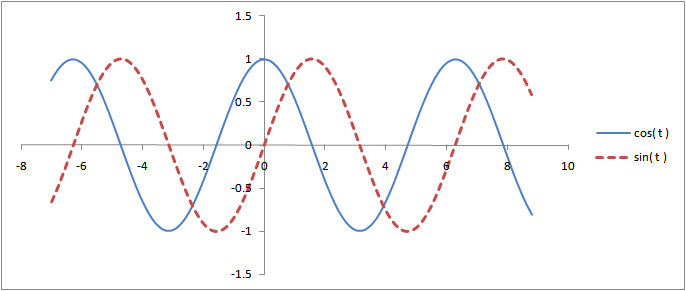
\includegraphics[width=\textwidth]
	         {images/cos_sin.png}}
	  \caption{\label{fig:complex:1} Graphs of cosine and sine }
\end{figure}


Note that some references use the word ``wavelength" instead of ``period"\index{Wavelength}. This is because they are considering equations like $y = \cos(x)$ where the independent variable $x$ represents distance. We are considering the independent variable to be time: so it is appropriate to use the word ``period'' instead.

Of course, there are cosine and sine waves with different periods. However, in this section  we will \emph{only}  be looking at cosine and sine waves with period $2\pi$. We re-emphasize:  all the cosine and sine waves in this chapter (and any that you use in the homework problems) have period $2 \pi$.

Now we can create other waves by using the cosine as a ``parent function''. For instance, the graph of
$y = A  \cos ( t + \theta) $ where $A > 0$
is similar to the graph of $y = \cos(t)$, with the following differences:

\begin{itemize}
\item
The amplitude is $A$
\item
The \term{phase shift}\index{Phase shift} (relative to the cosine curve) is $\theta$. 
\end{itemize}

%Changed 1/22/12 JW
\begin{rem} 
\begin{itemize}
\item
You may have studied ``parent functions'' in high school, and if so you may remember that the graph of $y = f(t+c)$ is shifted to the \emph{left} compared to the graph of $y = f(t)$.  It follows that a positive phase shift will shift the graph to the \emph{left}, while a negative phase shift will shift it to the \emph{right} (see Figure~\ref{fig:complex:2}).\footnote{ You should be careful when you encounter the term ``phase shift'' in other books, because some books define a positive phase shift as moving the graph to the \emph{right}. This is not wrong: it's just different terminology.}
\item 
If the variable $t$ is considered as time, then $y = A  \cos ( t + \theta) $ is \emph{advanced} by $\theta$ (corresponding to a left shift of the graph), while $y = A  \cos ( t - \theta) $ is \emph{delayed} by $\theta$ (corresponding to a right shift of the graph).  
\end{itemize}
\end{rem}
%replaces:
%\begin{rem} 
%Be careful about the term ``phase shift''\index{Phase shift}. Some books define the phase of $y = A  \cos ( t + \theta) $ as $-\theta$ and not $\theta$ -- this is because the graph of $y = A  \cos ( t + \theta) $ includes the point $(-\theta,1)$.  If the variable $t$ is considered as time, then $y = A  \cos ( t + \theta) $ is \emph{advanced} by $\theta$ (corresponding to a left shift of the graph), while $y = A  \cos ( t - \theta) $ is \emph{delayed} by $\theta$ (corresponding to a right shift of the graph).
%\end{rem}
%1/22/12
 
\begin{figure}[htb]
	   \center{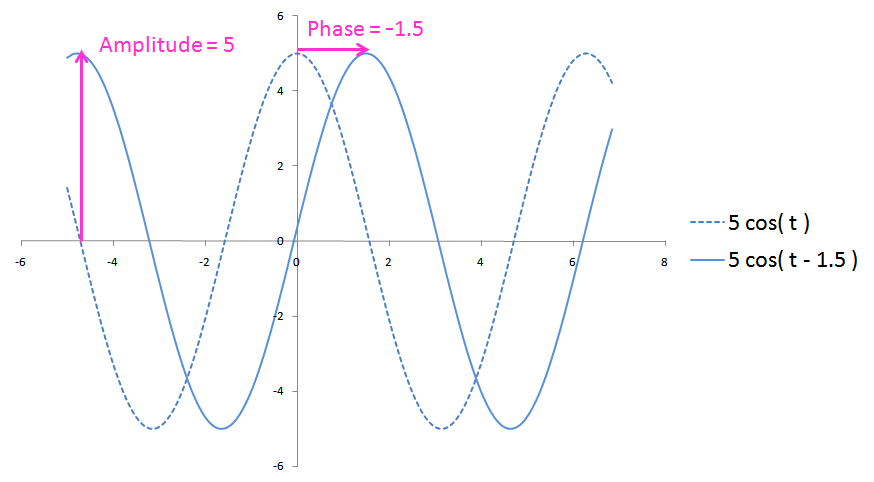
\includegraphics[width=\textwidth]
	         {images/ampl_phase.png}}
	  \caption{\label{fig:complex:2} Cosine wave with amplitude and phase shift}
\end{figure}

\begin{exercise}{41}
Sketch the function $y = 1.5 \cos(t + \pi/3)$. Label the amplitude and phase shift on your graph.
\end{exercise}

\begin{exercise}{wave1}
Give the equation of a cosine wave with amplitude 7 and phase shift $-\pi$/2. Graph the function. How is this function related to a sine wave?
\end{exercise}

\begin{exercise}{waves}
Give the equation of a cosine wave with amplitude $1/2$ and phase shift $2\pi$. Graph the function. How is this wave related to the original cosine wave with phase shift 0?
\end{exercise}

\begin{exercise}{42}
\begin{enumerate}[(a)]
\item
Sketch the function $y = \sin(t)$.
\item
Find three different  choices of $A,\theta$ such that 
$ \sin(t) = A  \cos (t + \theta)$.  What are the possible values of $A$?
\hyperref[sec:complex:hints]{(*Hint*)}

\end{enumerate}
\end{exercise}

\noindent
In summary, amplitude and phase are two important properties of cosine and sine waves; and in fact the amplitude and phase uniquely determine the actual wave, as you saw in Exercises~\ref{exercise:complex:wave1} and \ref{exercise:complex:waves}. Now earlier in this chapter, we saw a different mathematical object that was characterized by amplitude and phase. Naturally, we're referring to the complex numbers.  We will now make a deep connection between these two types of mathematical objects that, on the surface, are very different.

Recall that the \emph{real part} of the complex number $z = a + bi$ is $a$, and the \emph{imaginary part} is $b$. We also use the notation Re$[z]$ to denote the real part of the complex number $z$, and the notation Im$[z]$ to denote the imaginary part.

\begin{exercise}{43}
Show that Re$ [A  \cis\theta \cdot \cis( t)]  = A  \cos ( t +  \theta). $
\hyperref[sec:complex:hints]{(*Hint*)}
 \end{exercise}

\begin{exercise}{44}
Show that Im$ [A \cis\theta \cdot \cis (t)] = A \sin (t + \theta). $
\end{exercise}

\noindent
The previous two exercises show that: 

\begin{itemize}
\item
A cosine wave with amplitude $A$ and phase shift $\theta$ can be represented  as the real part of  the complex number $A \cis\theta$ times the complex function $\cis(t)$.
\item
A sine wave with amplitude $A$ and phase shift $\theta$ can be represented  as the imaginary part of  the complex number $A \cis\theta$ times the complex function $\cis(t)$.
\end{itemize}

\noindent
We may also understand this situation in terms of two-dimensional vectors with the help of Figure \ref{fig:complex:3}. We've already shown how complex numbers can be seen as two-dimensional vectors: in particular, the complex number $\cis\theta$ is identified with $\cos\theta$\textbf{i} + $\sin\theta$\textbf{j}. As $t$ varies, the point $\cis(t+\theta)$ moves around the unit circle,and the real part of $\cis(t + \theta)$ is the projection of the moving point onto the $x$-axis.  In other words, the cosine wave on the right side of Figure \ref{fig:complex:3} tells us the vector's horizontal distance to the $y$-axis as a function of time $t$.

\begin{figure}[htb]
	   \center{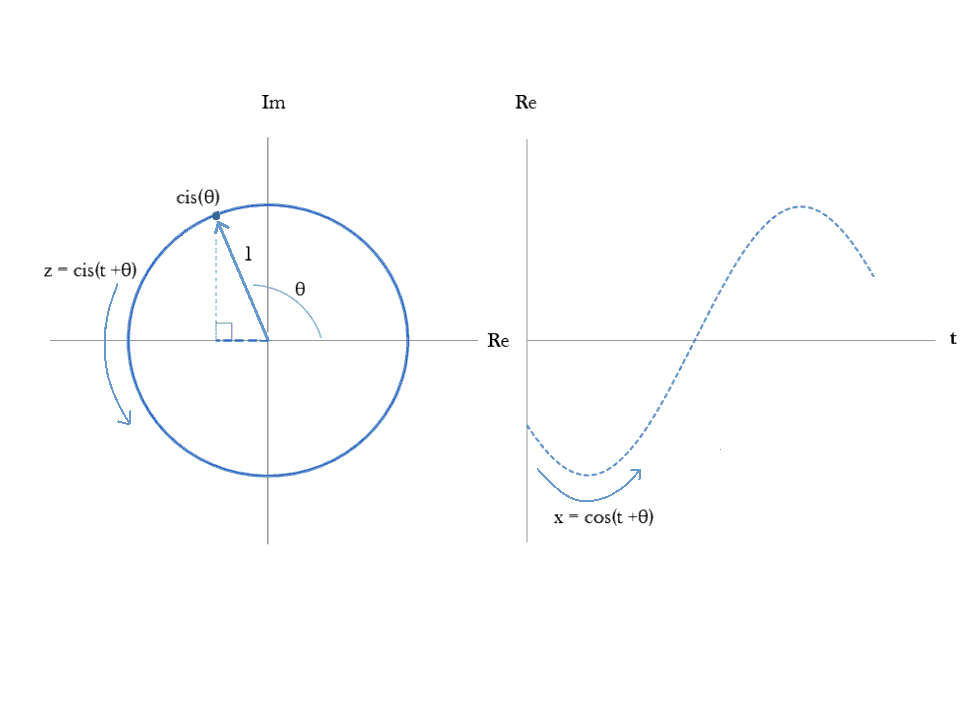
\includegraphics[width=\textwidth]
	         {images/phasors.png}}
	  \caption{\label{fig:complex:3} Graphs of the vector representation and the wave representation of cosine }
\end{figure}

Now when two waves cross each other they produce a wave of a different shape--we may see this in water waves at the beach or pool (or physics class). This is called {\bf \emph{wave superposition}}\index{Wave superposition}. We will now see how complex numbers make it easy to compute the shape of this new wave.

\begin{exercise}{45}
\begin{enumerate}[(a)]
\item
Using $\cis \theta = \cos \theta + i\sin \theta$, complete the following argument by filling in the blanks:
\begin{align*} 
2 \cos(t + \pi/2) + 2 \cos(t - 5\pi/6) &= \text{Re}[2 \cis (t + \pi/2)] + \text{Re}[\underline{~<1>~})]\\
&= \text{Re}[2 \cis (t) \cdot \cis(\pi/2)] + \textrm{Re}[\underline{~<2>~})]\\
&= \text{ Re} \left[\left(\, 2 \cis(\pi/2) + 2 \cis(-5\pi/6) \, \right) \cdot \underline{~<3>~}) \right] 
\end{align*}
\item
Convert $2 \cis(\pi/2)$ and $2 \cis(-5\pi/6)$ to cartesian form, and find the sum. Then convert back to polar form.
\item
Use your result in (b) to simplify the right-hand side of (a).
\item
Your result in (c) shows that the sum of the two cosine waves  $2\cos(t + \pi/2)$ and $2 \cos(t - 5\pi/6)$ is also equal to a cosine wave.  Find the amplitude and phase shift of the sum. Is the amplitude equal to the sum of the amplitudes? Explain.
\end{enumerate}
\end{exercise}

Let us summarize our findings:
\begin{itemize}
\item
Associated with each sine or cosine wave is a complex number $A \cis( \theta) $ such that $A$ is the amplitude and $\theta$ is the phase shift of the wave. This complex number is called the \term{phasor}\index{Phasor} associated with the wave.
\item
The sum of two sine or cosine waves is also equal to a cosine wave
\item
The amplitude and phase shift of the sum of two cosine waves may be obtained by adding the phasors of the two constituent cosine waves.
\end{itemize}

\begin{exercise}{46}
A radio antenna receives three cosine-wave signals. The first signal has an amplitude of 4 and a phase shift of 0. The second has an amplitude of 3 and a phase shift of $\pi/2$. The third signal has an amplitude of 2 and a phase shift of $-\pi/3$.
\begin{enumerate}[(a)]
\item
On graph paper,  plot the three phasors corresponding to the three signals. (The three phasors are $4 \cis(0), 3 \cis(\pi/2),$ and $2 \cis(-\pi/3)$)
\item
Use your picture in (a) to graphically add the three phasors. (Remember how to add vectors:  add the $x$-components, and add the $y$-components.)
\item
Convert the three phasors to rectangular form, and add them together algebraically.
\item
Use your result from (c) to find the amplitude and phase shift of the sum of the three signals.
\end{enumerate}
\end{exercise}


\begin{exercise}{47}
As in the previous problem, a radio antenna receives three cosine-wave signals. The three signals have equal amplitude. The first signal have a phase shift of 0. The second has a phase shift of $2\pi/3$. The third signal has  a phase shift of $4\pi/3$.
\begin{enumerate}[(a)]
\item
 What is the amplitude of the sum of the three signals?
\item
What is the phase shift of the sum of the three signals?
\end{enumerate}
\end{exercise}

We hope that from the examples in this section, you may get some idea of how important complex numbers are in the study of signals. In fact, for many electrical engineers complex numbers are their ``bread and butter''. 


\subsection{Complex numbers and fractals: the Mandelbrot set} \label{sec:mandelbrot}
The intricate \emph{Mandelbrot set}\index{Mandelbrot set} (see Figure~\ref{mandelbrot}) is a beautiful application of complex numbers.
The Mandelbrot set is defined by means of \emph{iteration} of the function $f(z) = z^2 + c$. The definition is a little complicated: we show how it works using a couple of examples.

First consider $c=1$, so $f(z) = z^2 + 1$. We start with $z=0$, which gives $f(0) = 1$; and we iterate by evaluating the function on the result of the previous evaluation. So we compute $f(1) = 2, f(2) = 5, f(5) = 26, \ldots.$. It is clear that $|f(z)|$ is getting larger and larger after repeated iterations. 

On the other hand, if we use $c=i$ and start with $z=0$, we get $f(0) = i$ at first, and repeated iteration gives $f(i) = -1+i, f(-1+i) =- i, f(-i) = -1 + i, \ldots$ so that this time $|f(z)|$ doesn't continue to grow indefinitely after repeated iterations. 

The Mandelbrot set is defined to be the set of values $c$ for which the iterations of $f(z) = z^2 + c$ starting from $z=0$ do \emph{not} grow indefinitely upon iteration. Thus $i$ is in the Mandelbrot set, while $1$ is not. 

\begin{exercise}{mandelbrot}
Which of the following numbers is in the Mandelbrot set? \emph{Demonstrate} your answers.
\begin{multicols}{2}
\begin{enumerate}[(a)]
\item
$c = 0$
\item
$c = -1$
\item
$c = -i$
\item
$c = 1+i$
\end{enumerate}
\end{multicols}
\end{exercise}

\begin{exercise}{mandel2}
In the definition of the Mandelbrot set, we mentioned that you have to check whether the iterations ``grow indefinitely''. The question, is, How far do you have to check? We can actually give an answer:
\begin{enumerate}[(a)]
\item
Given any two complex numbers $z,w$, show that:
\begin{equation*}
|z + w| \le |z| + |w|.
\end{equation*}
This is called the \emph{triangle inequality}\index{triangle inequality! for complex numbers} for complex numbers (it is closely related to the `triangle inequality' for vectors). \hyperref[sec:complex:hints]{(*Hint*)}
\item
Prove the following variation of the triangle inequality:  Given two complex numbers $z,w$ then $|z| \ge |z-w| - |w|$.
\item
Suppose that $|c| < 2$, and suppose that $z \ge 2$. Use (b) to show  that $|z^2 + c| > |z|$.
\item
In order to guarantee that a number $c$ is in the Mandelbrot set, all we have to do is show that one of the iterates of the function $f(z) = z^2 + c$ is larger than a given positive number $r$.  What is the value of $r$?  
\end{enumerate}
\end{exercise}

\begin{figure}[hbt]  
\center{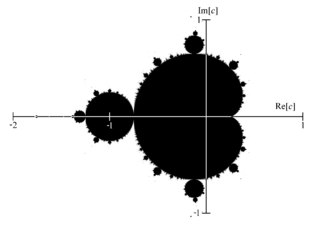
\includegraphics[width=5.in]
	         {images/mandelbrot.png}}
\caption{(\emph{Left}) The Mandelbrot set: the set itself is colored in maroon. The  set has delicate filaments that extend from the different bulb-shaped areas, which are outlined in lighter color.(\emph{Right}) Detail of the Mandelbrot set, along the top edge of the heart-shaped region shown in the figure at left. \label{mandelbrot}}
\end{figure}

\begin{exercise}{excel}(\emph{Programming exercise})
\begin{enumerate}[(a)]
\item
Write an Excel spreadsheet that can multiply two complex numbers. Put the real and imaginary parts of the first number in cells A1 and B1; Put the real and imaginary parts of the second number in cells C1 and D1; Put the real and imaginary parts of the result in cells E1 and F1. Use your sheet to compute $(3 + 4i)(7 - 8i)$.
\item
Copy your Excel sheet, and modify it to compute the square of a complex number. Put the real and imaginary parts of the first number in cells A1 and B1; Put the real and imaginary parts of the result in cells C1 and D1. Use your sheet to compute $(12 - 5i)^2$.
\item 
Copy and modify your Excel sheet to compute $z^2, (z^2)^2,((z^2)^2)^2, \ldots$ (20 number altogether) for a given complex number $z$. Put the real and imaginary parts of $z$ in cells A1 and B1; Put the real and imaginary parts of the results in columns C and D. Use your sheet with $z = 0.8 + 0.6i$. Plot the results as 20 points in the plane (use Scatter Plot). What do you notice about your numbers?
\item
 Modify your Excel sheet to compute the first 100 iterates of the function $f(z) = z^2 + c$ for given complex numbers $z,c$ (see Exercise~\ref{exercise:complex:mandelbrot}). Put the real and imaginary parts of $z$ in cells A1 and B1; Put the real and imaginary parts of $c$ in cells A2 and B2; put the results in columns C and D. Using your sheet, determine which of the following numbers is in the Mandelbrot set: (i) $z = -1.04039 + 0.2509294i$; (ii) $c=-0.1155989 + 0.7639405i$.
\end{enumerate}
\end{exercise} 

\begin{exercise}
Using $c = -3/4 + 0.01$ compute the sequence for 100 iterations, and note the iteration at which the value exceeds 2.  Do the same thing for $c = -3/4 + 0.001$, but for 1000 iterations.  Do you see any relationship between your results and the value of $\pi$?
\end{exercise}